\documentclass[12pt]{article}
\usepackage[a4paper, margin=1in, headheight=14pt]{geometry}
\usepackage[utf8]{inputenc}
\usepackage[spanish]{babel}
\usepackage{tabularx}
\usepackage{graphicx}
\usepackage{float}
\usepackage{setspace}
\usepackage{anyfontsize}
\usepackage[toc,page]{appendix} % Remove toc,page to render wo appendix
\usepackage{hyperref}
\usepackage[table]{xcolor}
\usepackage{fancyhdr}
\usepackage{nameref}
\usepackage{datetime}
\usepackage{tikz}
\usepackage[11pt]{moresize}
\usepackage{enumerate}
\usepackage{etoolbox}


\usetikzlibrary{calc}
\newcommand\HRule{\rule{\textwidth}{1pt}}


\pagestyle{fancy}
\fancyhf{}
\fancyhead[LE,RO]{Grupo 4}
\fancyhead[RE,LO]{\nombredelproyecto}
\fancyfoot[CE,CO]{\leftmark}
\fancyfoot[LE,RO]{\thepage}

\renewcommand{\headrulewidth}{2pt}
\renewcommand{\footrulewidth}{1pt}



\newcommand{\nombredelproyecto}{\textbf{Diagramas de secuencia y de clases GUI}}
\setcounter{secnumdepth}{4}
\makeatletter
\renewcommand{\paragraph}{\@startsection{paragraph}{4}{0ex}%
    {-3.25ex plus -1ex minus -0.2ex}%
    {1.5ex plus 0.2ex}%
    {\normalfont\normalsize\bfseries}}
\makeatother

\title{\nombredelproyecto} 
\author{Jesús Abajo Magro \\
Alejandro Díaz Blázquez \\
Javier Fernández Gamo \\
Andrés Galbán Méndez \\
Alejandro Gómez Molano \\
Jaime Millán Ibáñez Archilla \\
Rodrigo Sosa Saez \\
Alejandro Barrachina Argudo}


\date{\today}

\begin{document}
\begin{titlepage}


    \makeatletter
    \centering
    \vspace*{6\baselineskip}

    %------------------------------------------------
    %	Title
    %------------------------------------------------


    {\huge \underbar{\nombredelproyecto}\par} % Title

    %------------------------------------------------
    %	Subtitle
    %------------------------------------------------

    Ingeniería del software\\
    Ingeniería informática e ingeniería de computadores

    \vspace*{3\baselineskip} % Whitespace under the subtitle


    \begin{figure}[H]
        \centering
        
\includegraphics[width=0.5\textwidth]{images/Banqueo.png}
    \end{figure}
    %------------------------------------------------
    %	Editor(s)
    %------------------------------------------------


    \vspace{0.75\baselineskip} % Whitespace before the editors
    \begin{flushright}
        \small\@author\\ % Editor list
    \end{flushright}


    \vspace{0.5\baselineskip} % Whitespace below the editor list


    \vfill % Whitespace between editor names and publisher logo

    \vspace{0.3\baselineskip} % Whitespace under the publisher logo

    2020 % Publication year
    \makeatother
\end{titlepage}

\tableofcontents
\newpage

\section{Introducción} %INTRODUCCION
En este documento se muestran los diagramas de secuencia y los diagramas de clase de las interfaces gráficas de la aplicación "Banqueo".

\section{Interfaces Gráficas} %INTERFACES GRAFICAS
En esta sección se muestran los diagramas de clases de las interfaces gráficas de la aplicación, con sus respectivos componentes.

\subsection{Interfaz Gráfica Cuentas}
\begin{figure}[H]
    \centering
    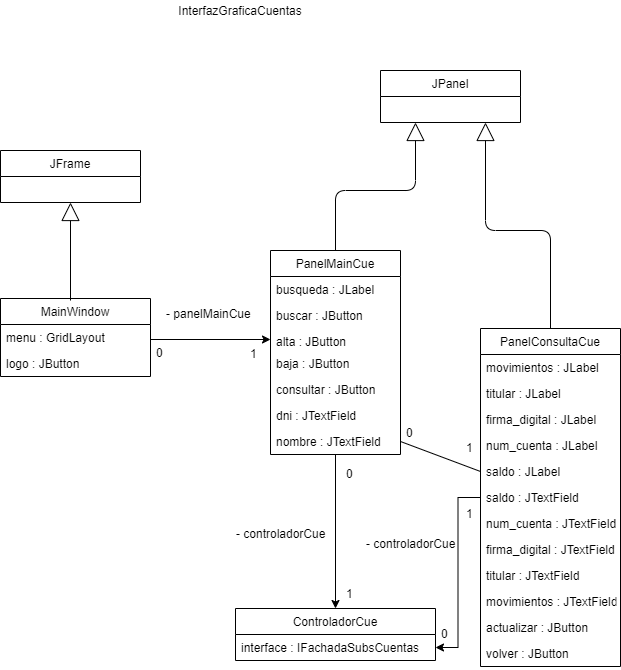
\includegraphics[width=0.8\textwidth]{images/InterfazGraficaCuentasFinal.png}
\end{figure}

\subsection{Interfaz Gráfica Tarjetas}
\begin{figure}[H]
    \centering
    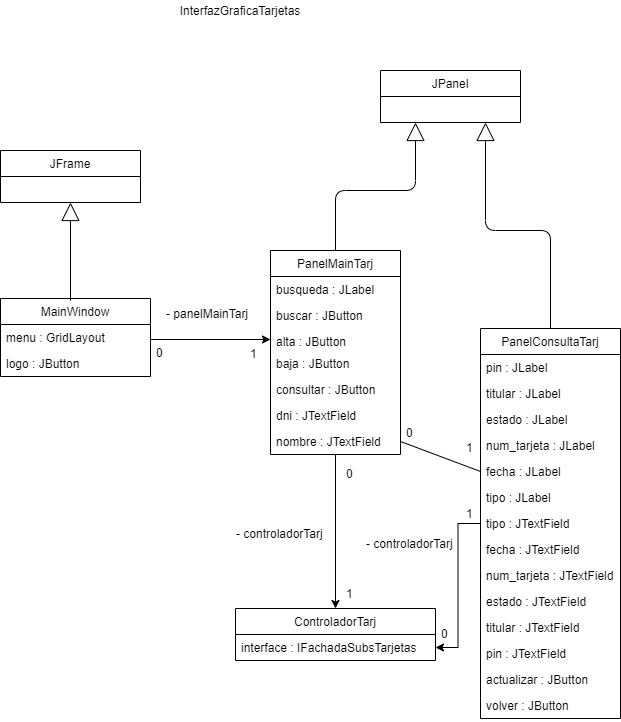
\includegraphics[width=0.8\textwidth]{images/InterfazGraficaTarjetasFinal.png}
\end{figure}

\subsection{Interfaz Gráfica Prestamos}
\begin{figure}[H]
    \centering
    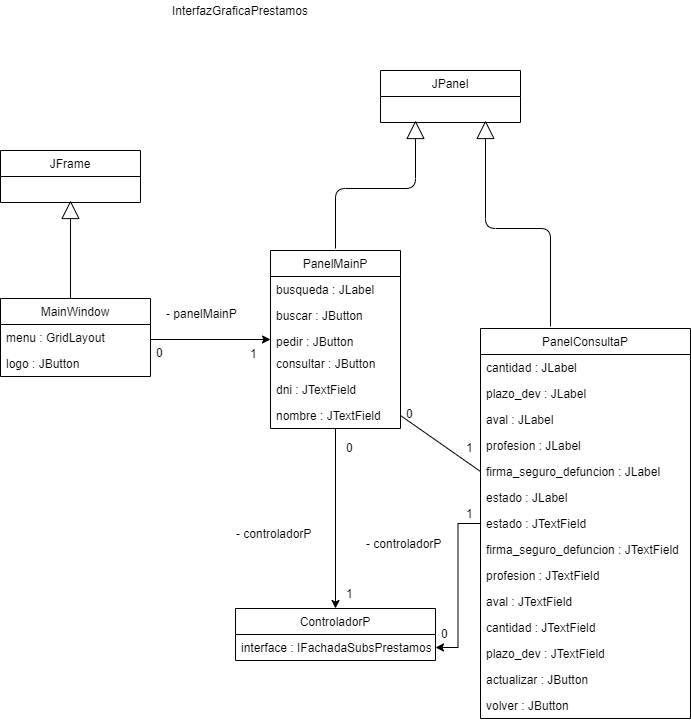
\includegraphics[width=0.8\textwidth]{images/InterfazGraficaPrestamosFinal.png}
\end{figure}

\subsection{Interfaz Gráfica Usuarios}
\begin{figure}[H]
    \centering
    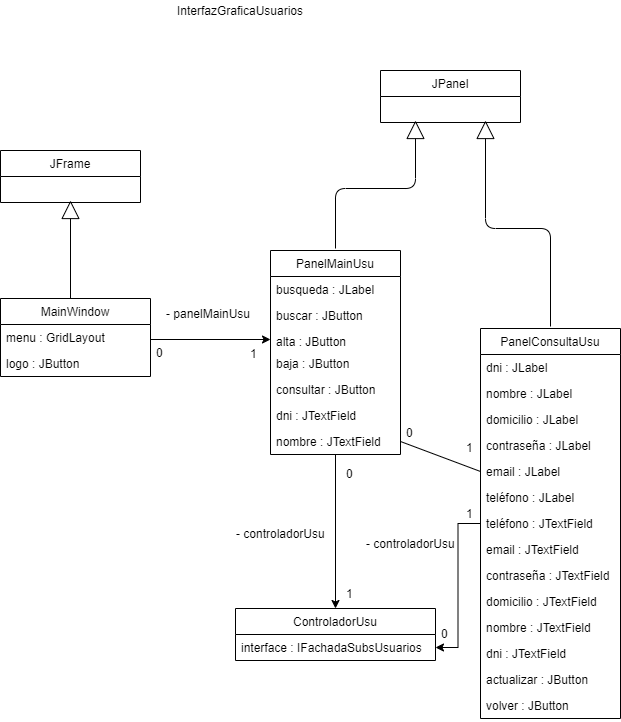
\includegraphics[width=0.8\textwidth]{images/InterfazGraficaUsuariosFinal.png}
\end{figure}

\newpage
\section{Diagramas de secuencia} %DIAGRAMAS DE SECUENCIA
En esta sección se muestran los diagramas de secuencia de los 4 subsistemas que existen en la aplicación: Usuarios, Cuentas, Préstamos y Tarjetas.
\subsection{Iniciar sesión}
Diagrama para la funcionalidad de iniciar sesión, que comprueba si los datos son correctos para poder acceder a la aplicación, y de serlo, en qué modo hacerlo.
\begin{figure}[H]
    \centering
    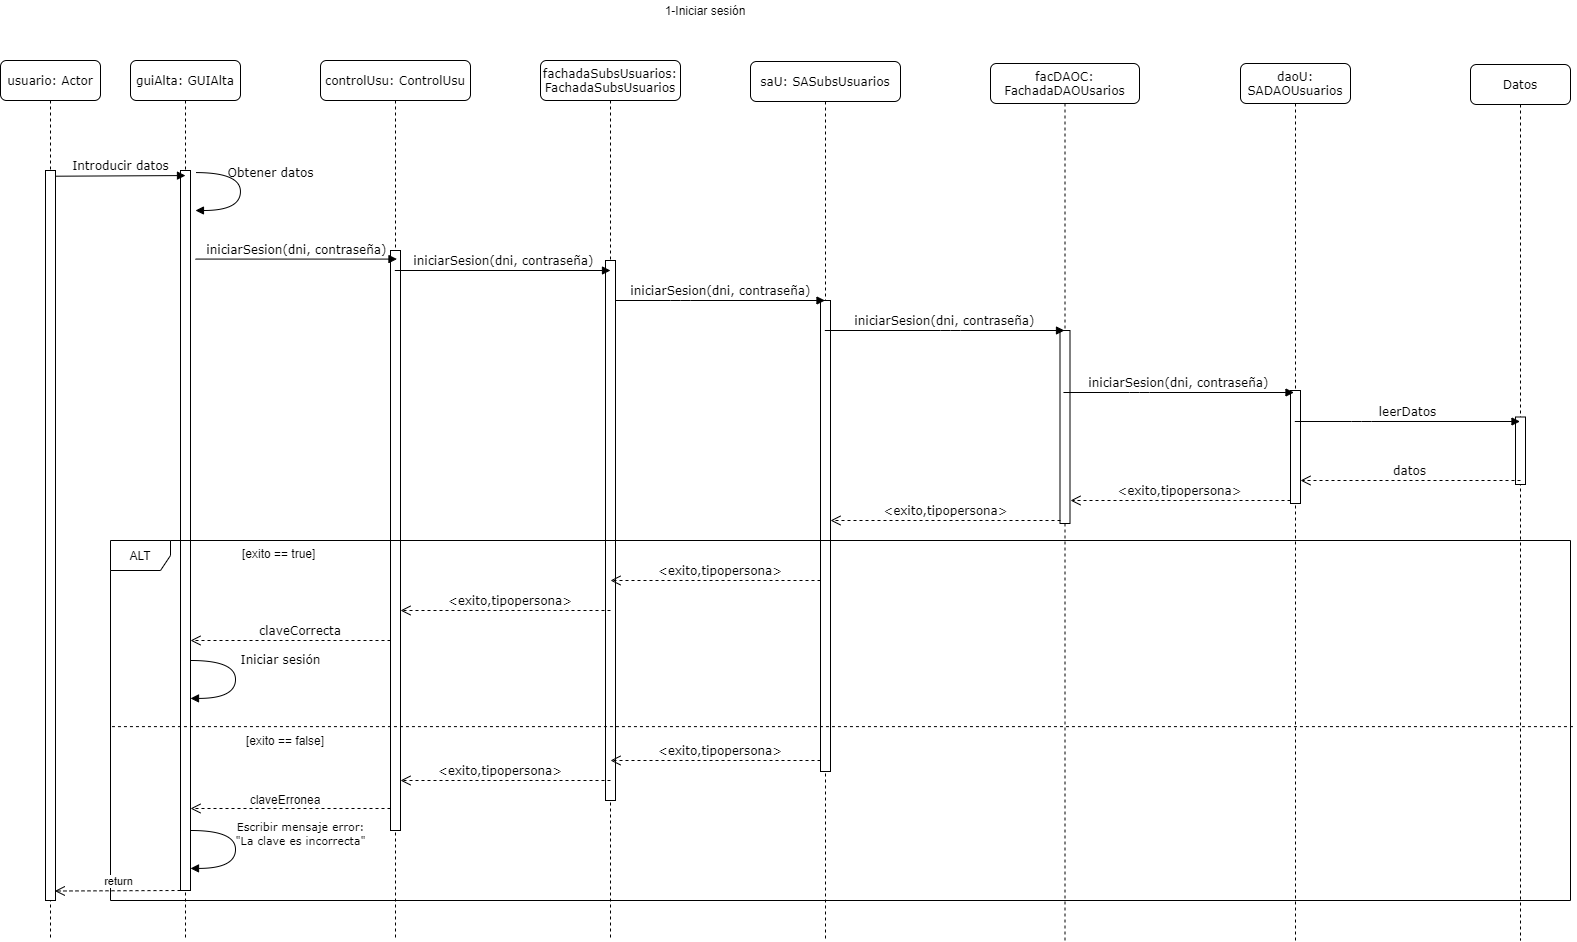
\includegraphics[width=0.8\textwidth]{images/1-iniciarSesionFinal.png}
\end{figure}
\subsection{Cerrar sesión}
Diagrama para la funcionalidad de cerrar sesión.
\begin{figure}[H]
    \centering
    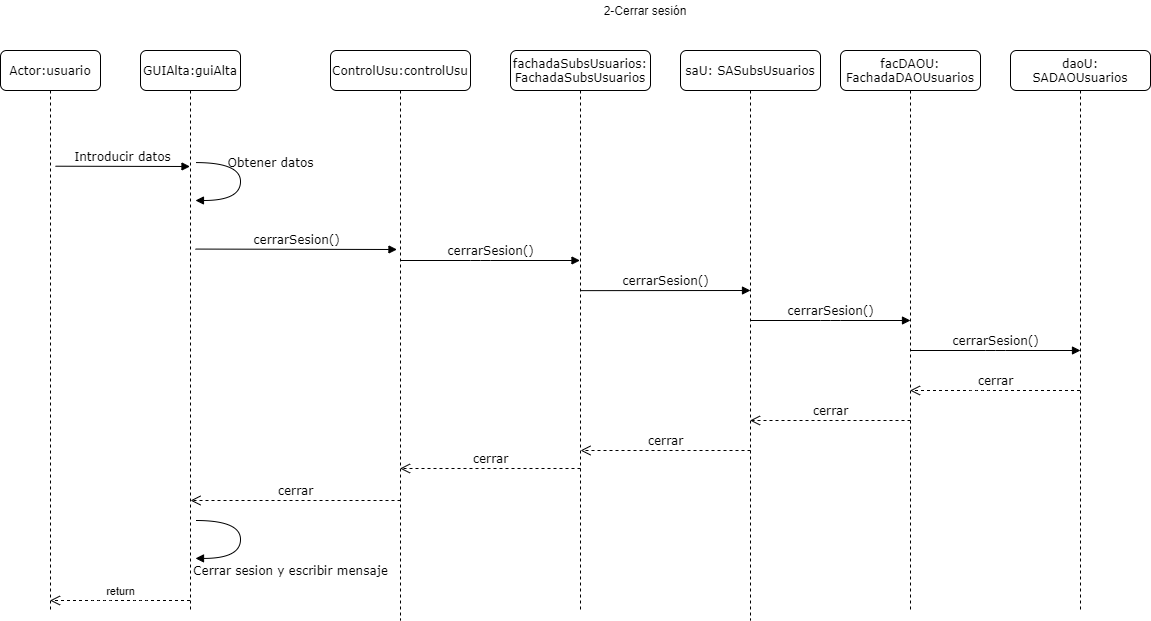
\includegraphics[width=0.4\textwidth]{images/2-CerrarSesionFinal.png}
\end{figure}
\subsection{Añadir cuenta}
Diagrama para la funcionalidad de crear cuenta, que accede a la base de datos para guardarla.
\begin{figure}[H]
    \centering
    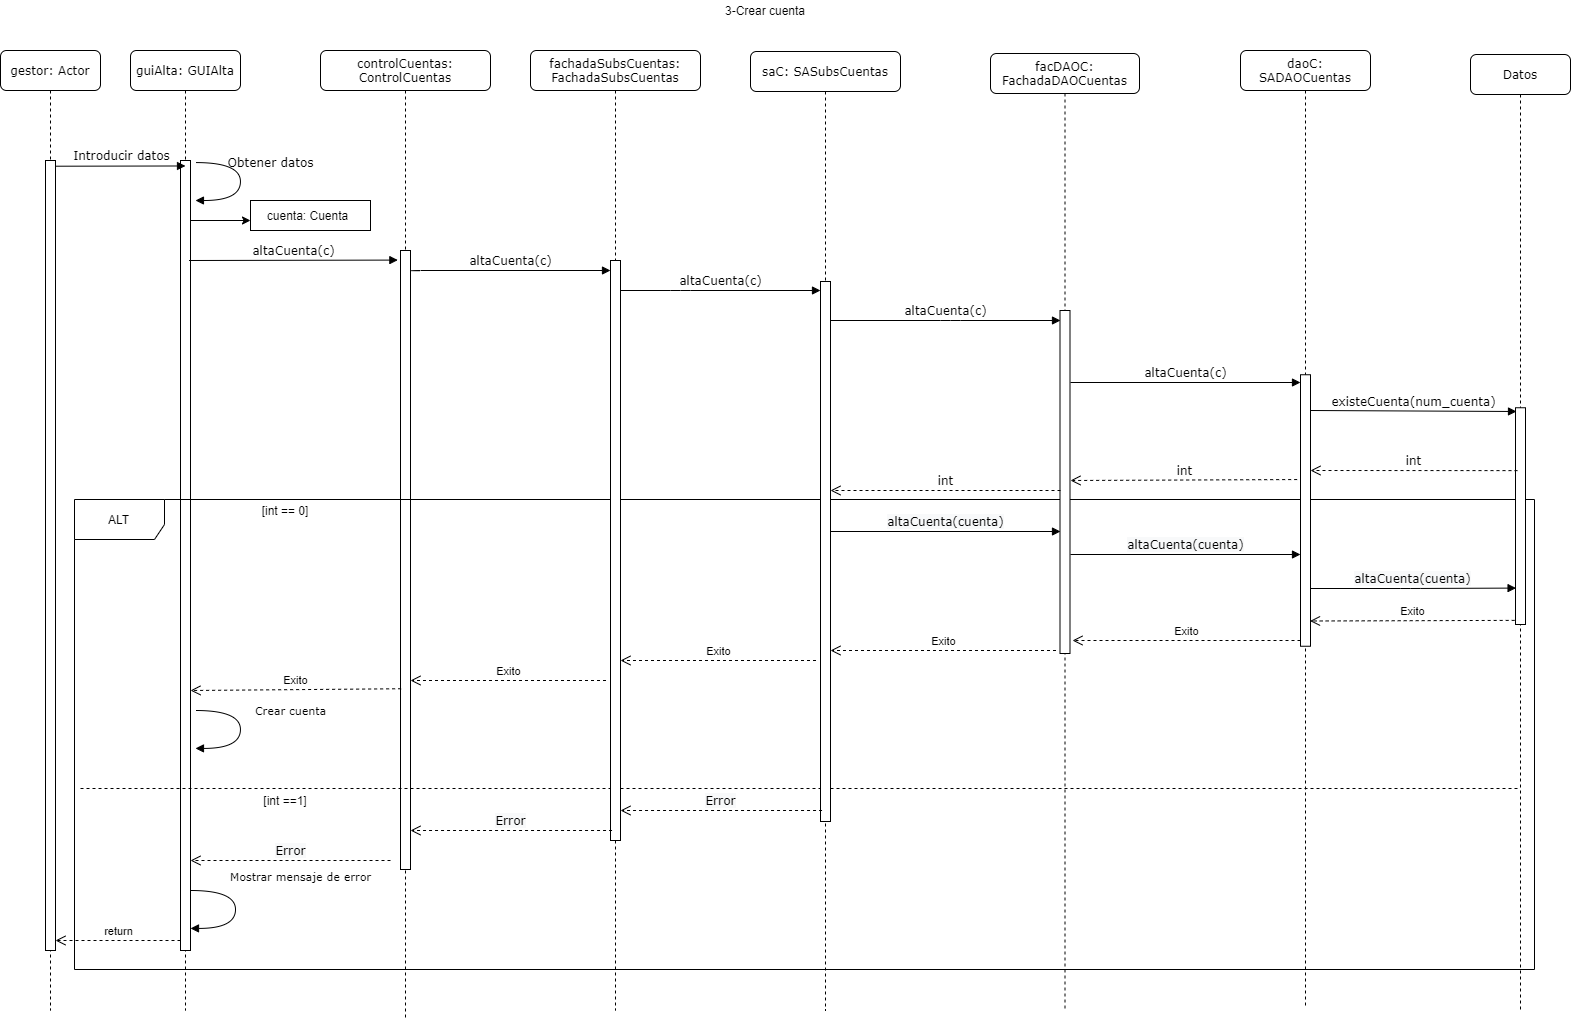
\includegraphics[width=0.8\textwidth]{images/3-crear_cuenta.png}
\end{figure}
\subsection{Eliminar cuenta}
Diagrama para la funcionalidad de eliminar cuenta, previamente comprobando si existe en la base de datos.
\begin{figure}[H]
    \centering
    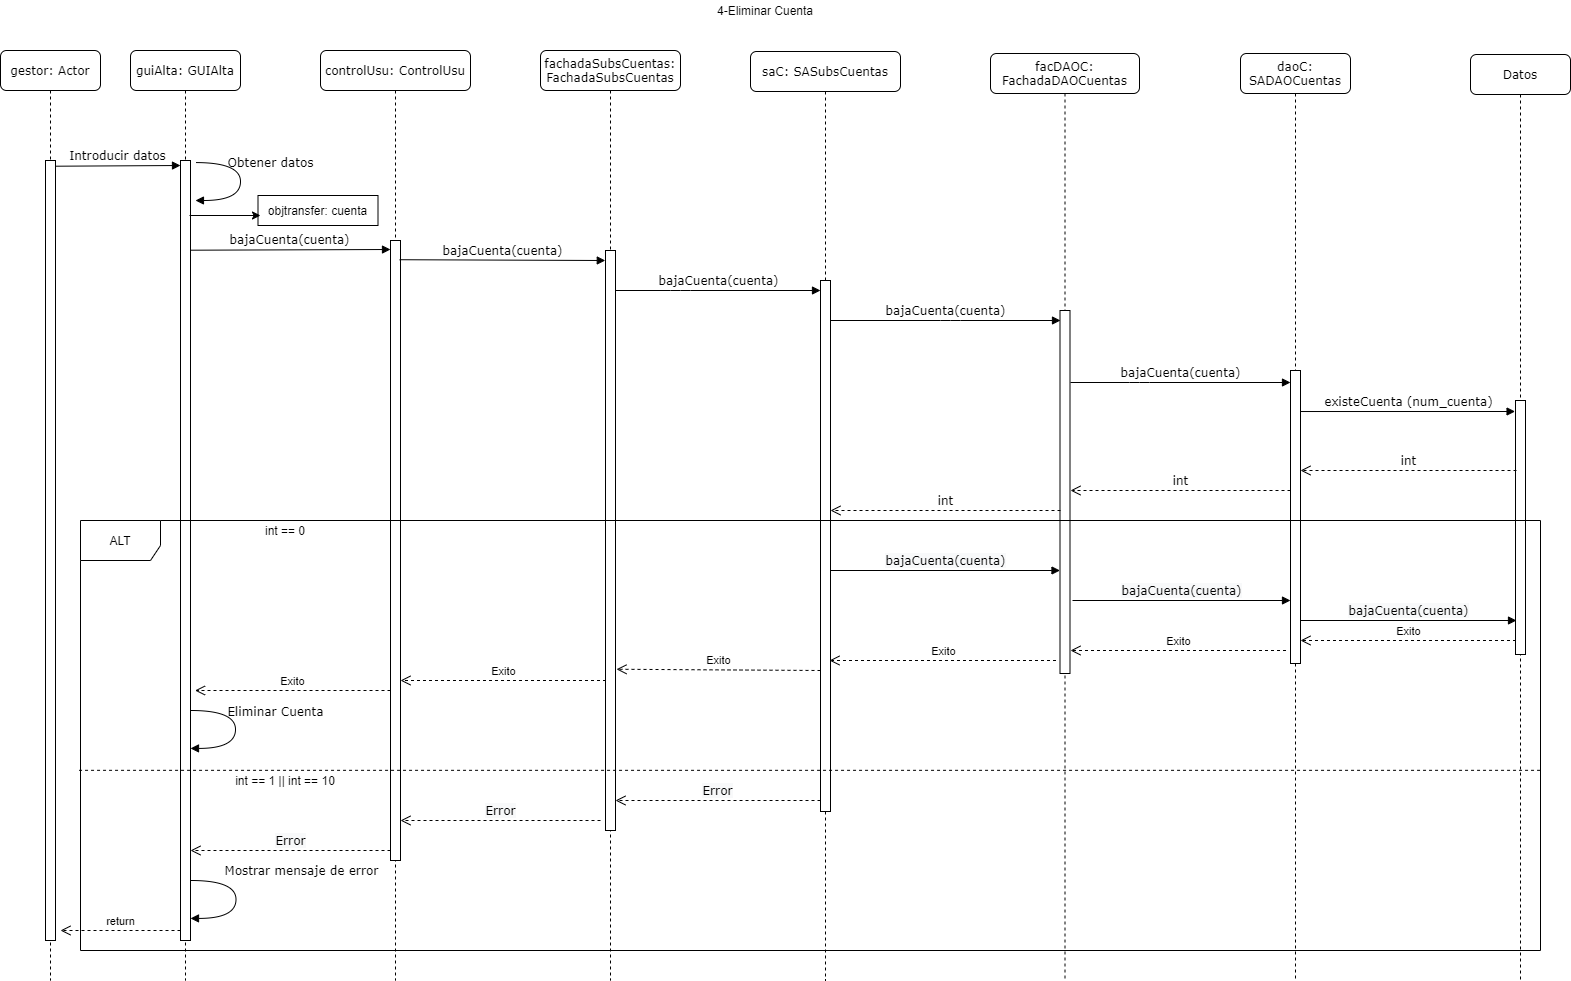
\includegraphics[width=0.8\textwidth]{images/eliminar_cuenta.png}
\end{figure}
\subsection{Consultar cliente}
Diagrama para la funcionalidad de buscar cliente en la base de datos.
\begin{figure}[H]
    \centering
    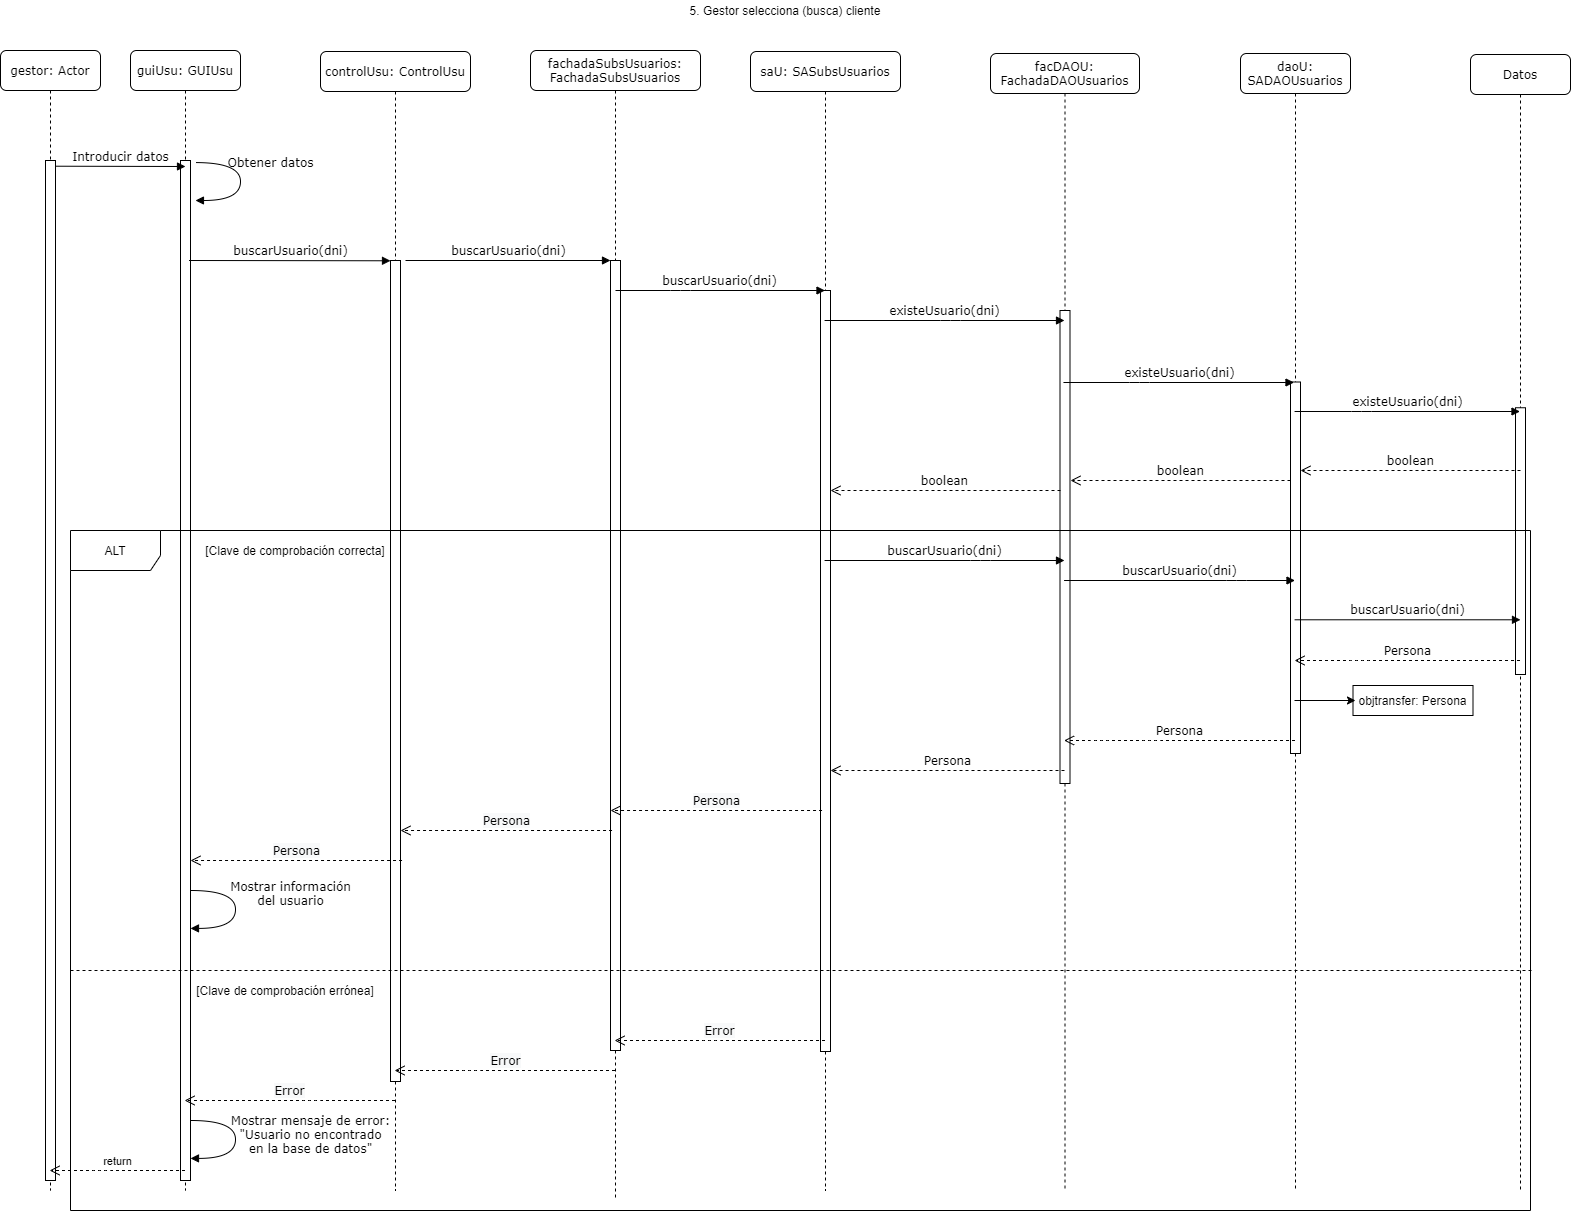
\includegraphics[width=0.8\textwidth]{images/gestor_selecciona_cliente_consultar_5.png}
\end{figure}
\subsection{Añade préstamo}

\begin{figure}[H]
    \centering
    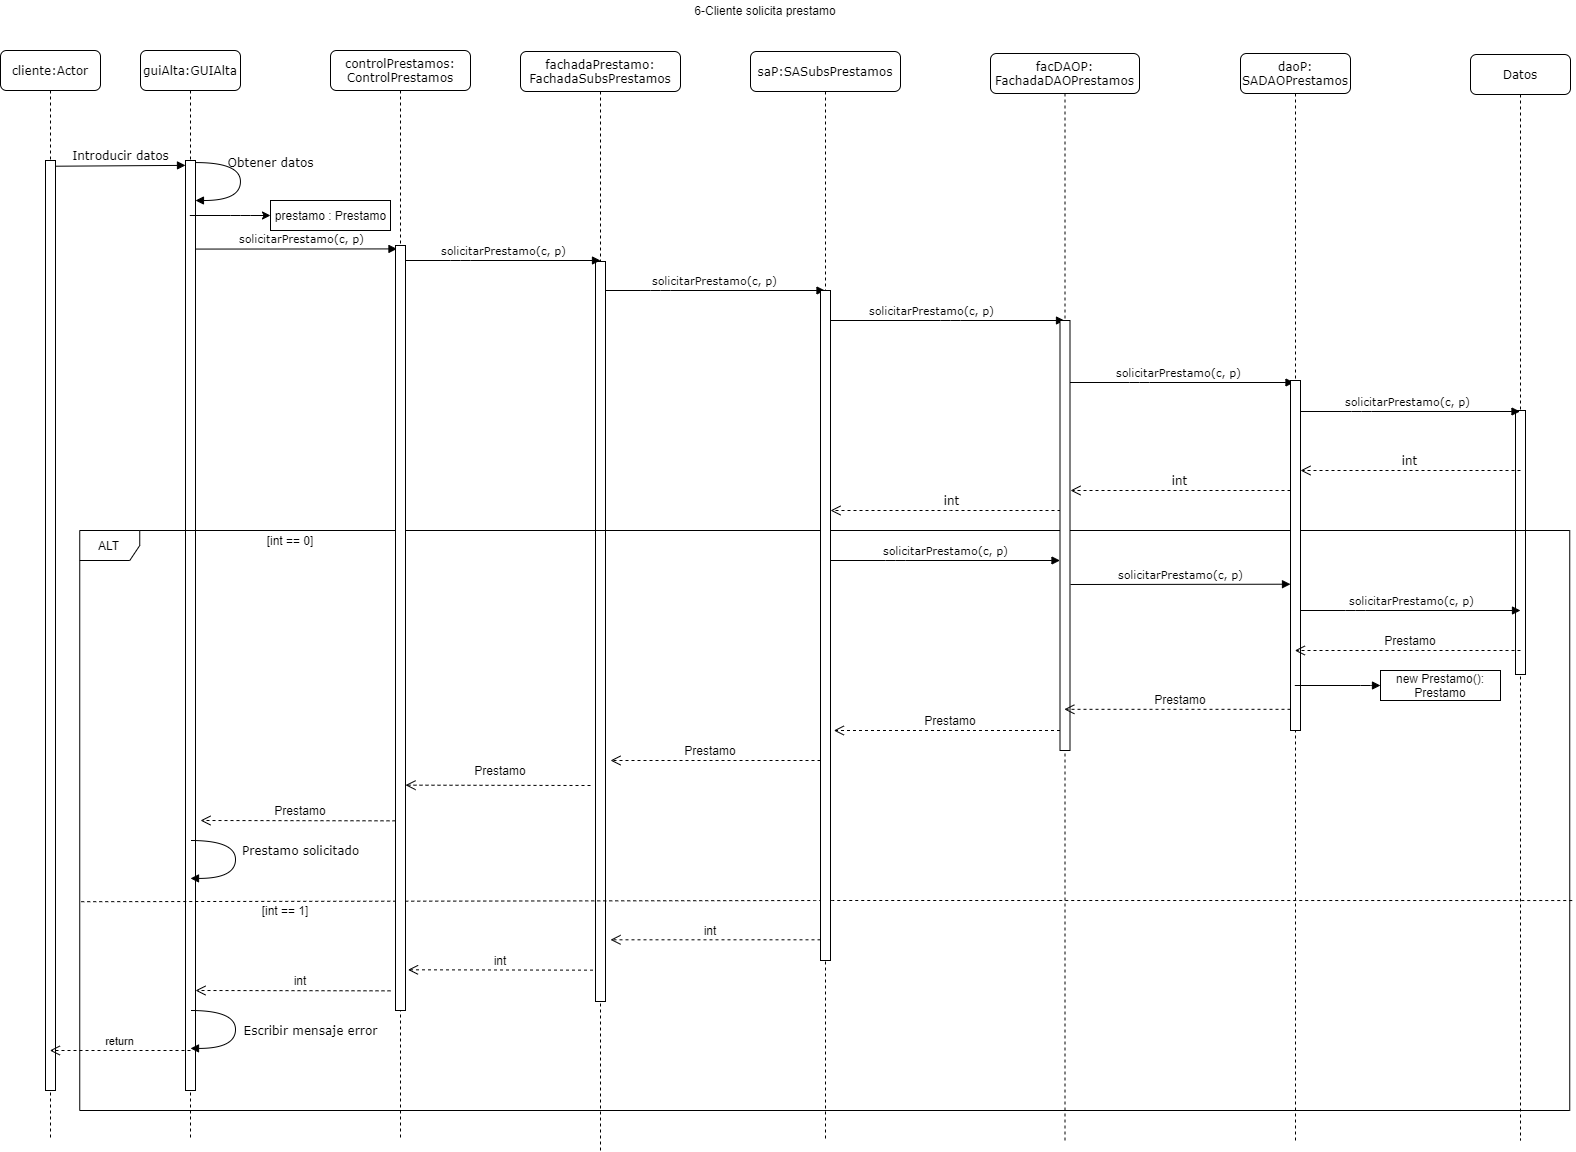
\includegraphics[width=0.8\textwidth]{images/ClienteSolicitaPrestamo2.png}
\end{figure}
\subsection{Modificar tarjeta}
\begin{figure}[H]
    \centering
    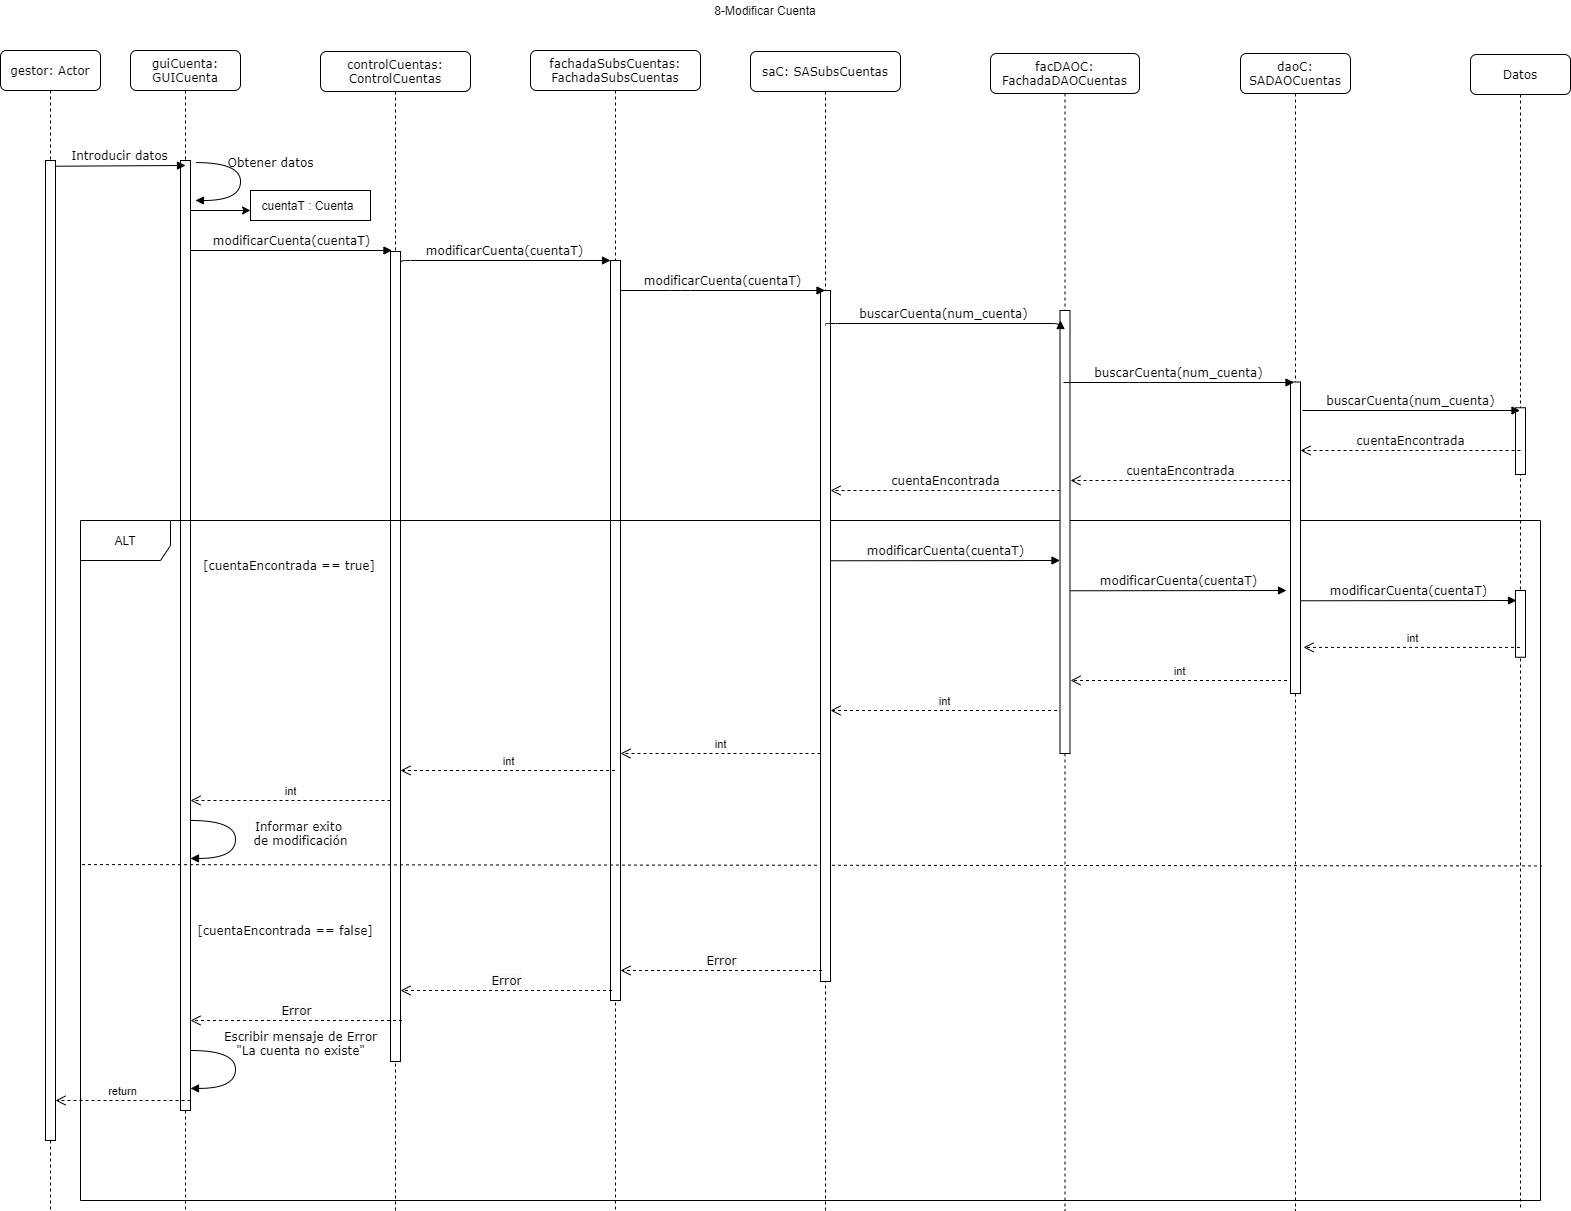
\includegraphics[width=0.8\textwidth]{images/7-Gestor_modifica_tarjeta1.png}
\end{figure}
\subsection{Modificar cuenta}
\begin{figure}[H]
    \centering
    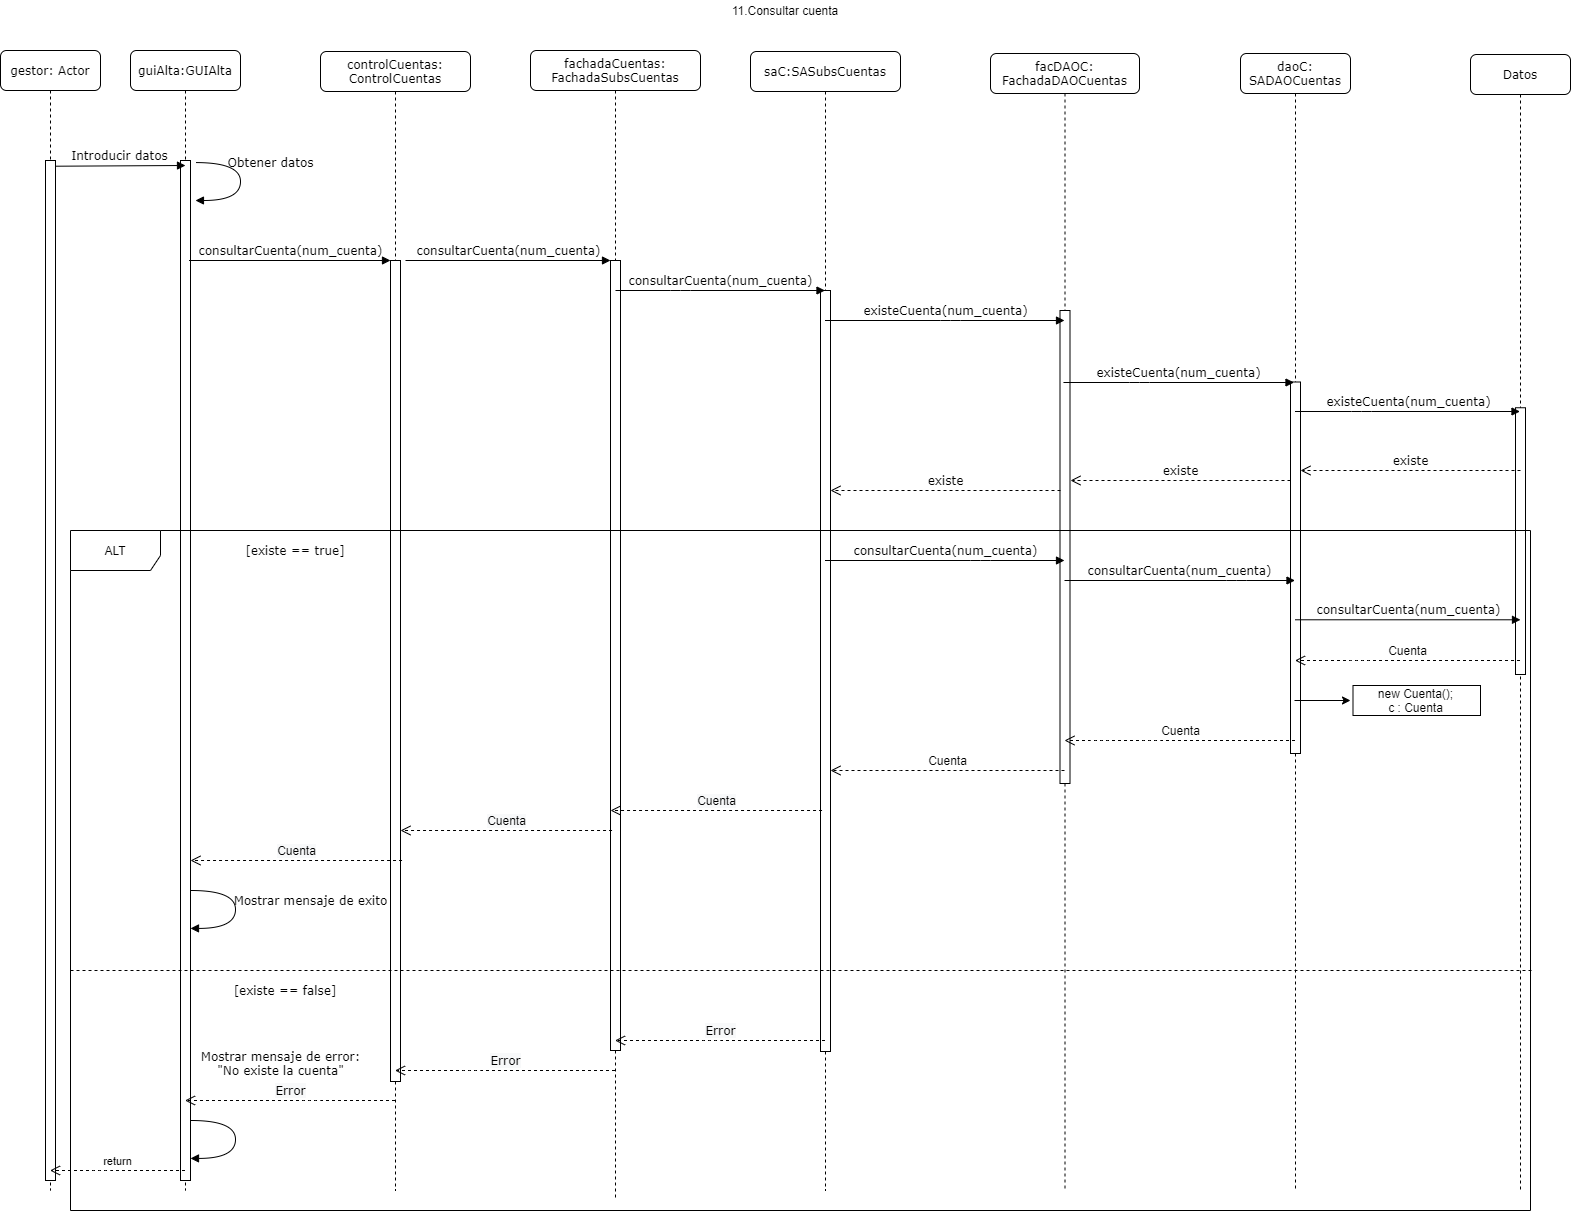
\includegraphics[width=0.8\textwidth]{images/8-Gestor_modifica_cuenta3.png}
\end{figure}
\subsection{Modificar préstamo}
\begin{figure}[H]
    \centering
    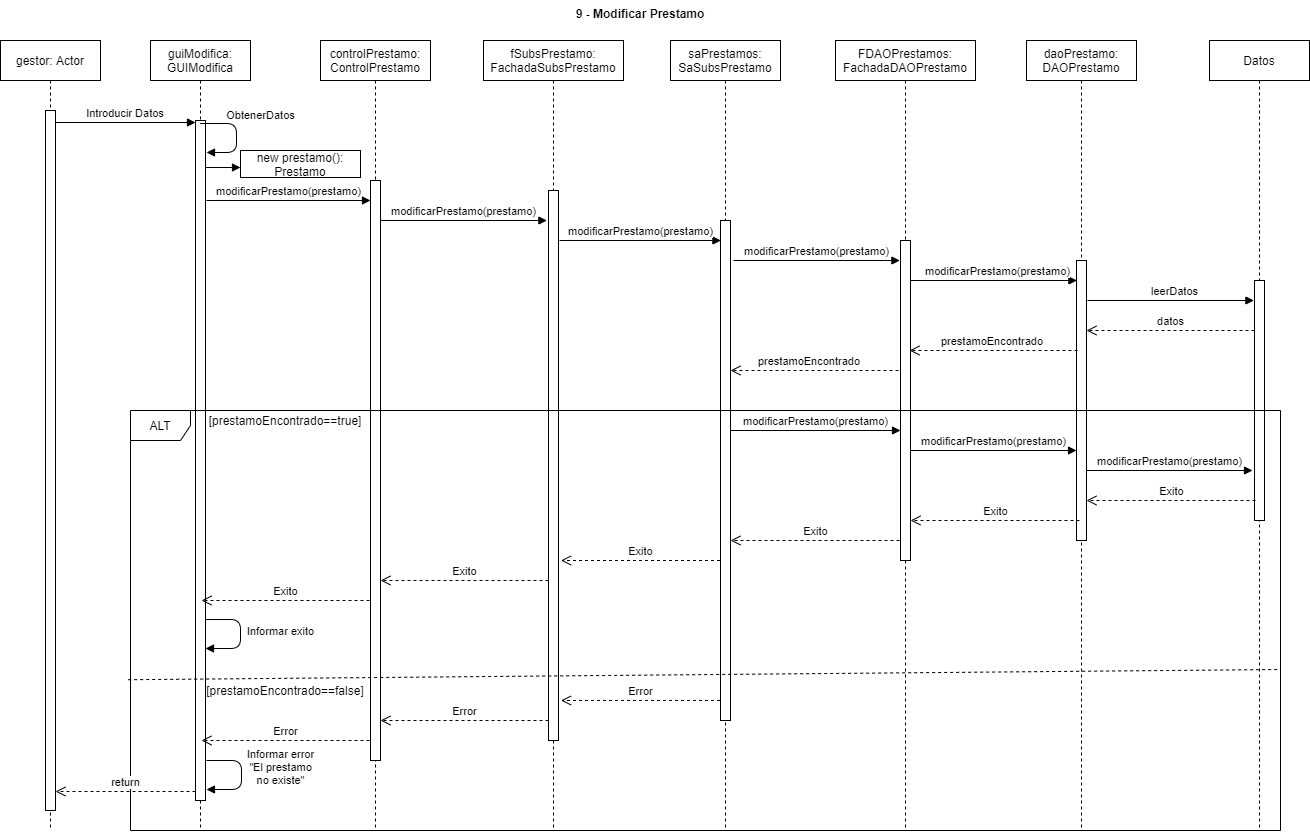
\includegraphics[width=0.8\textwidth]{images/9-GestorModificaPrestamoFinal.png}
\end{figure}
\subsection{Modificar usuario}
\begin{figure}[H]
    \centering
    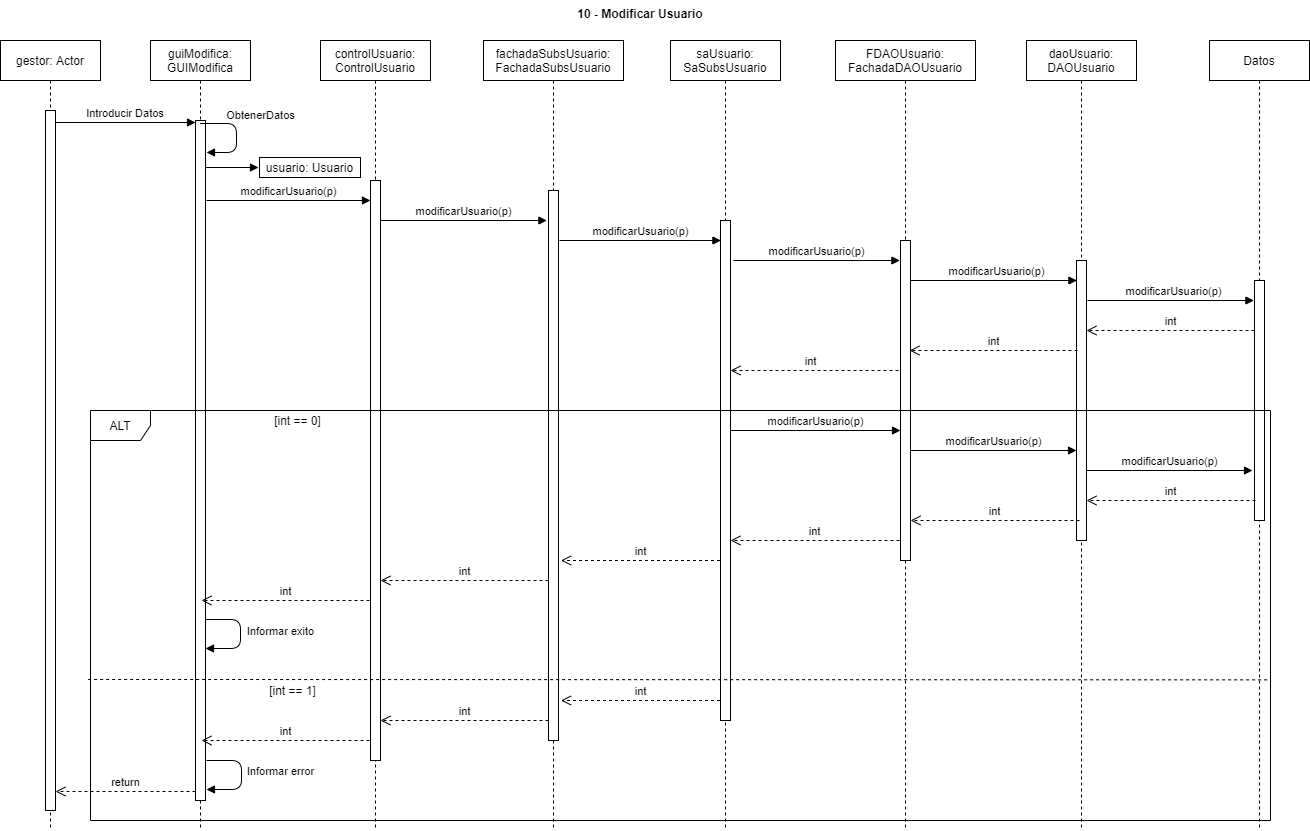
\includegraphics[width=0.8\textwidth]{images/10._ModificarUsuario.png}
\end{figure}
\subsection{Consultar cuenta}
\begin{figure}[H]
    \centering
    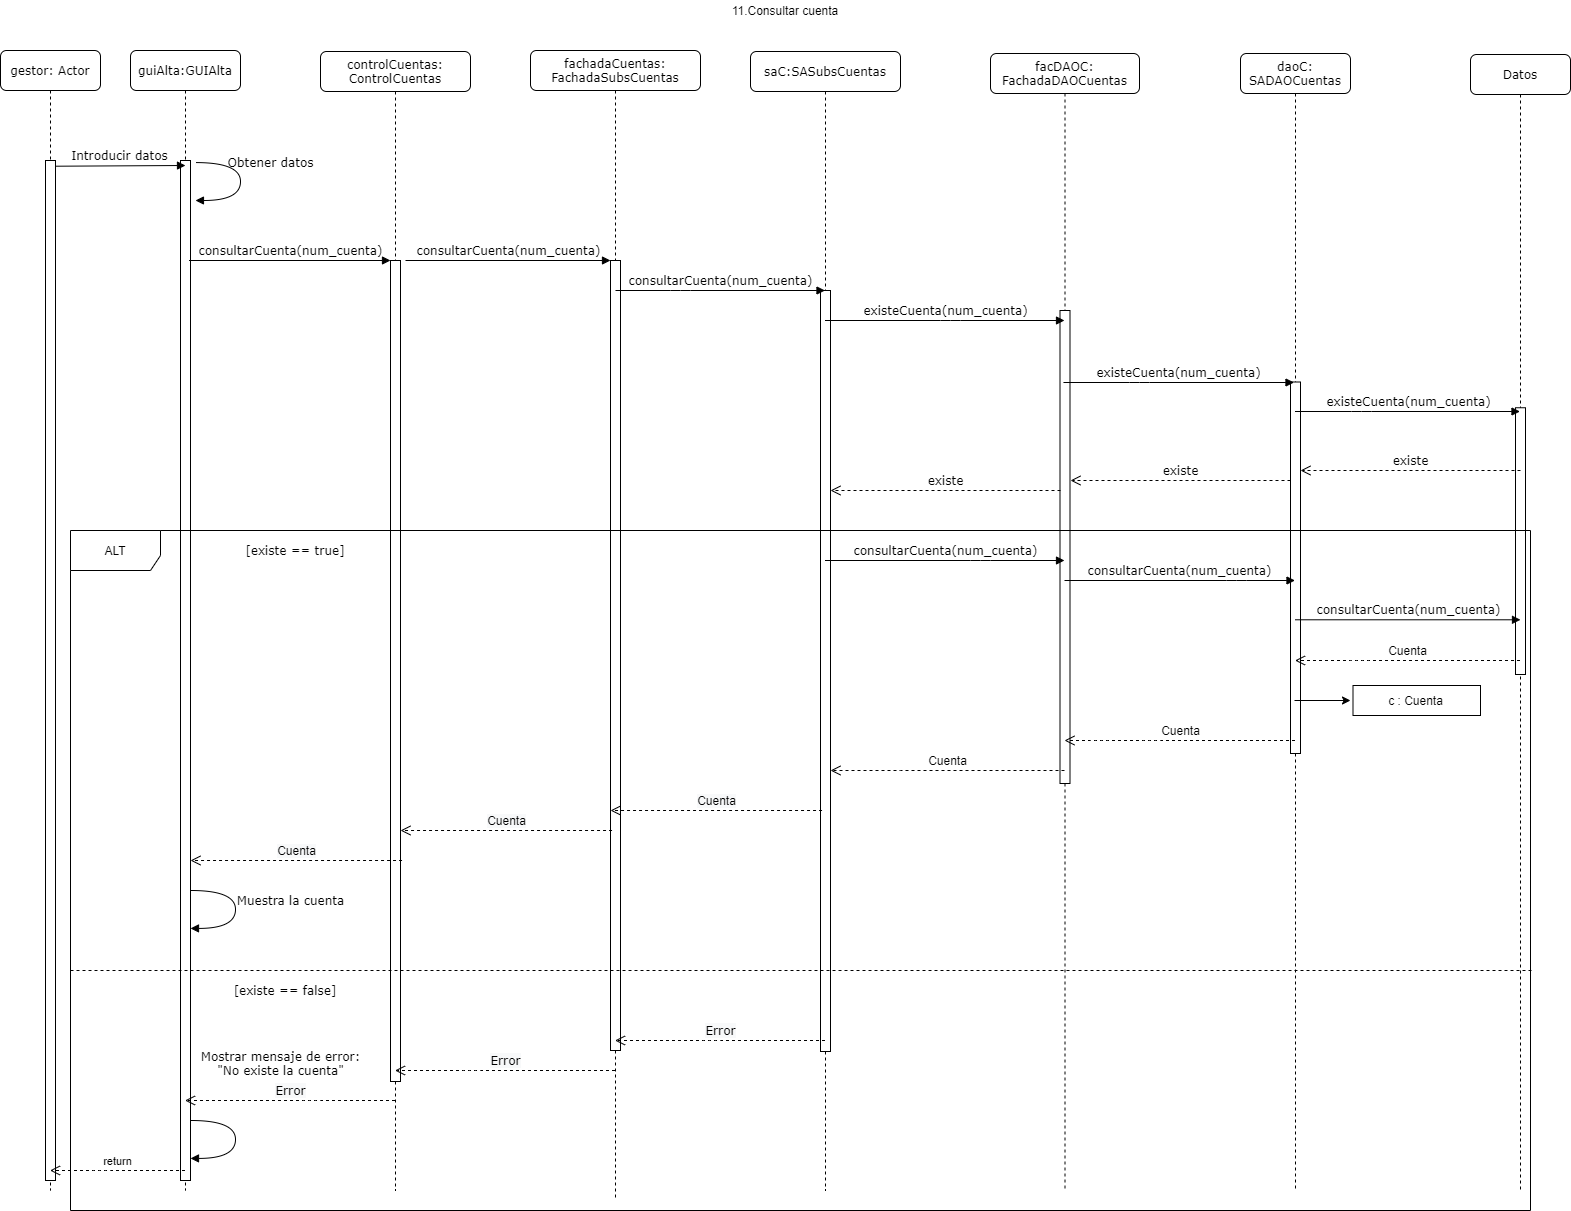
\includegraphics[width=0.8\textwidth]{images/ConsultaCuenta.png}
\end{figure}
\subsection{Consultar préstamo}
\begin{figure}[H]
    \centering
    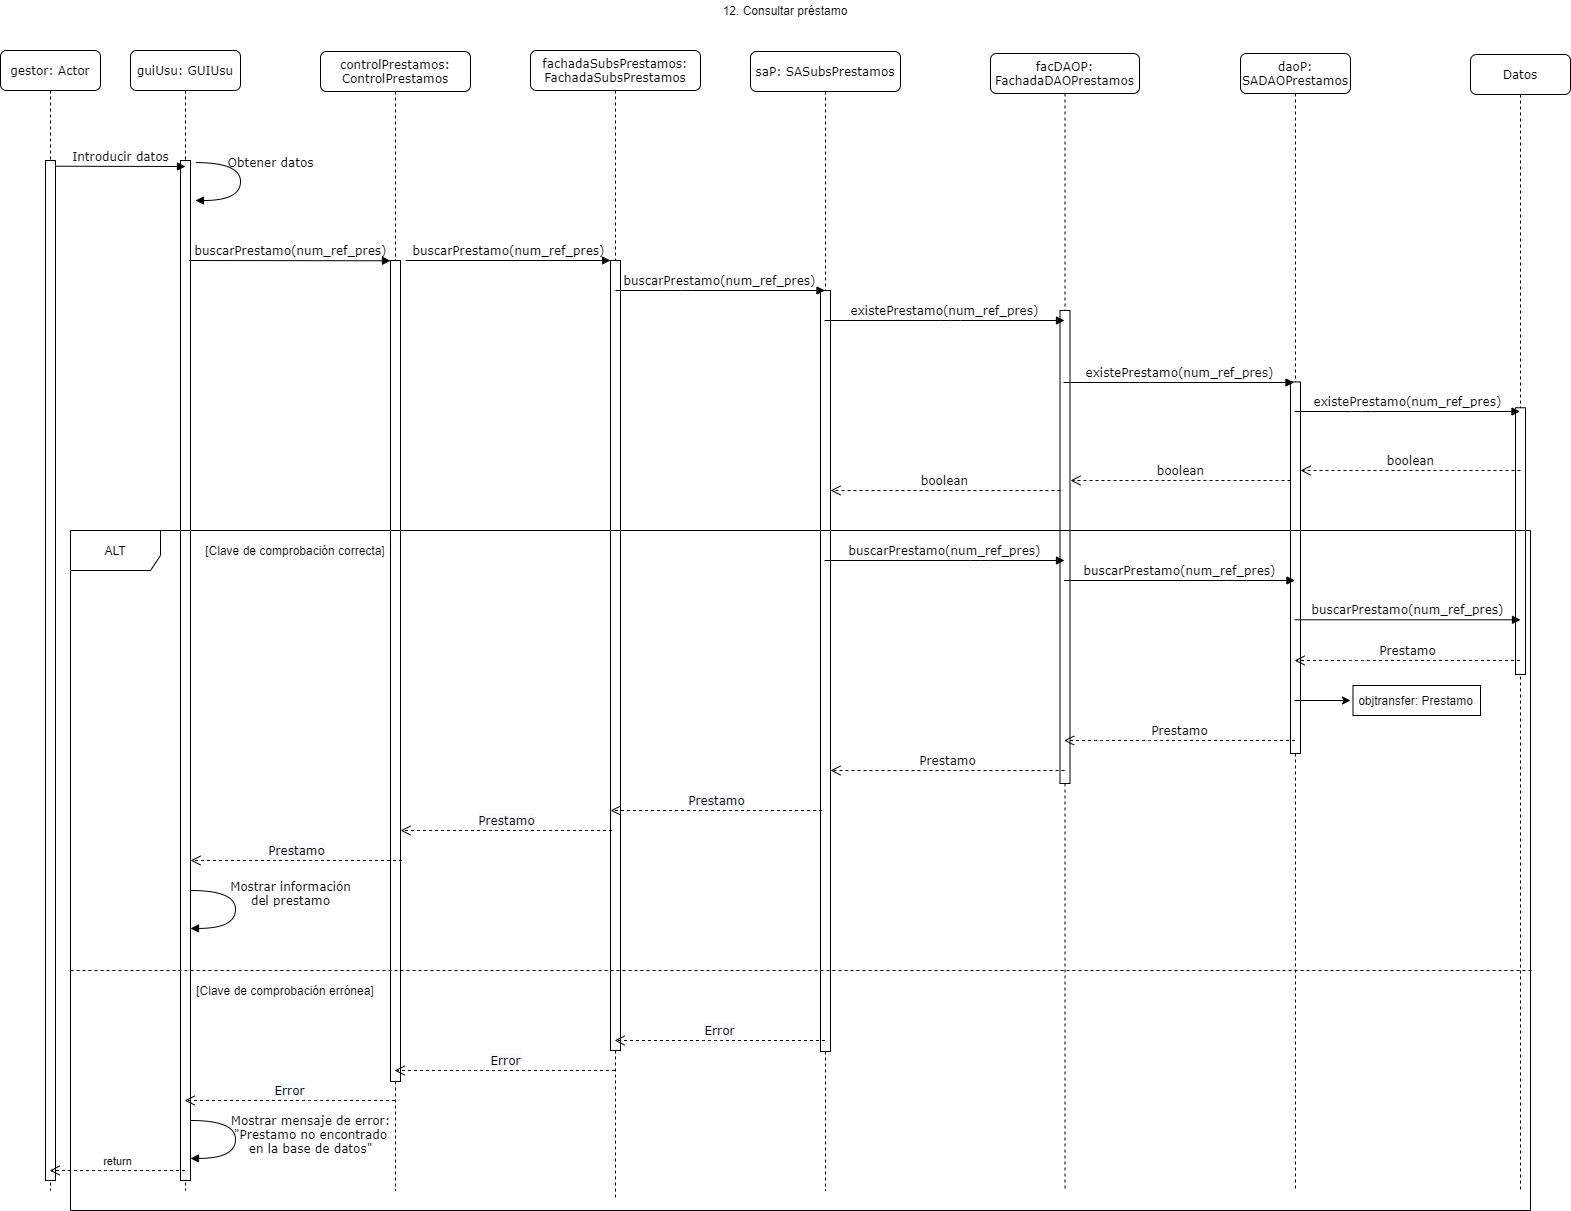
\includegraphics[width=0.8\textwidth]{images/consultar_prestamo.png}
\end{figure}
\subsection{Consultar tarjeta}
\begin{figure}[H]
    \centering
    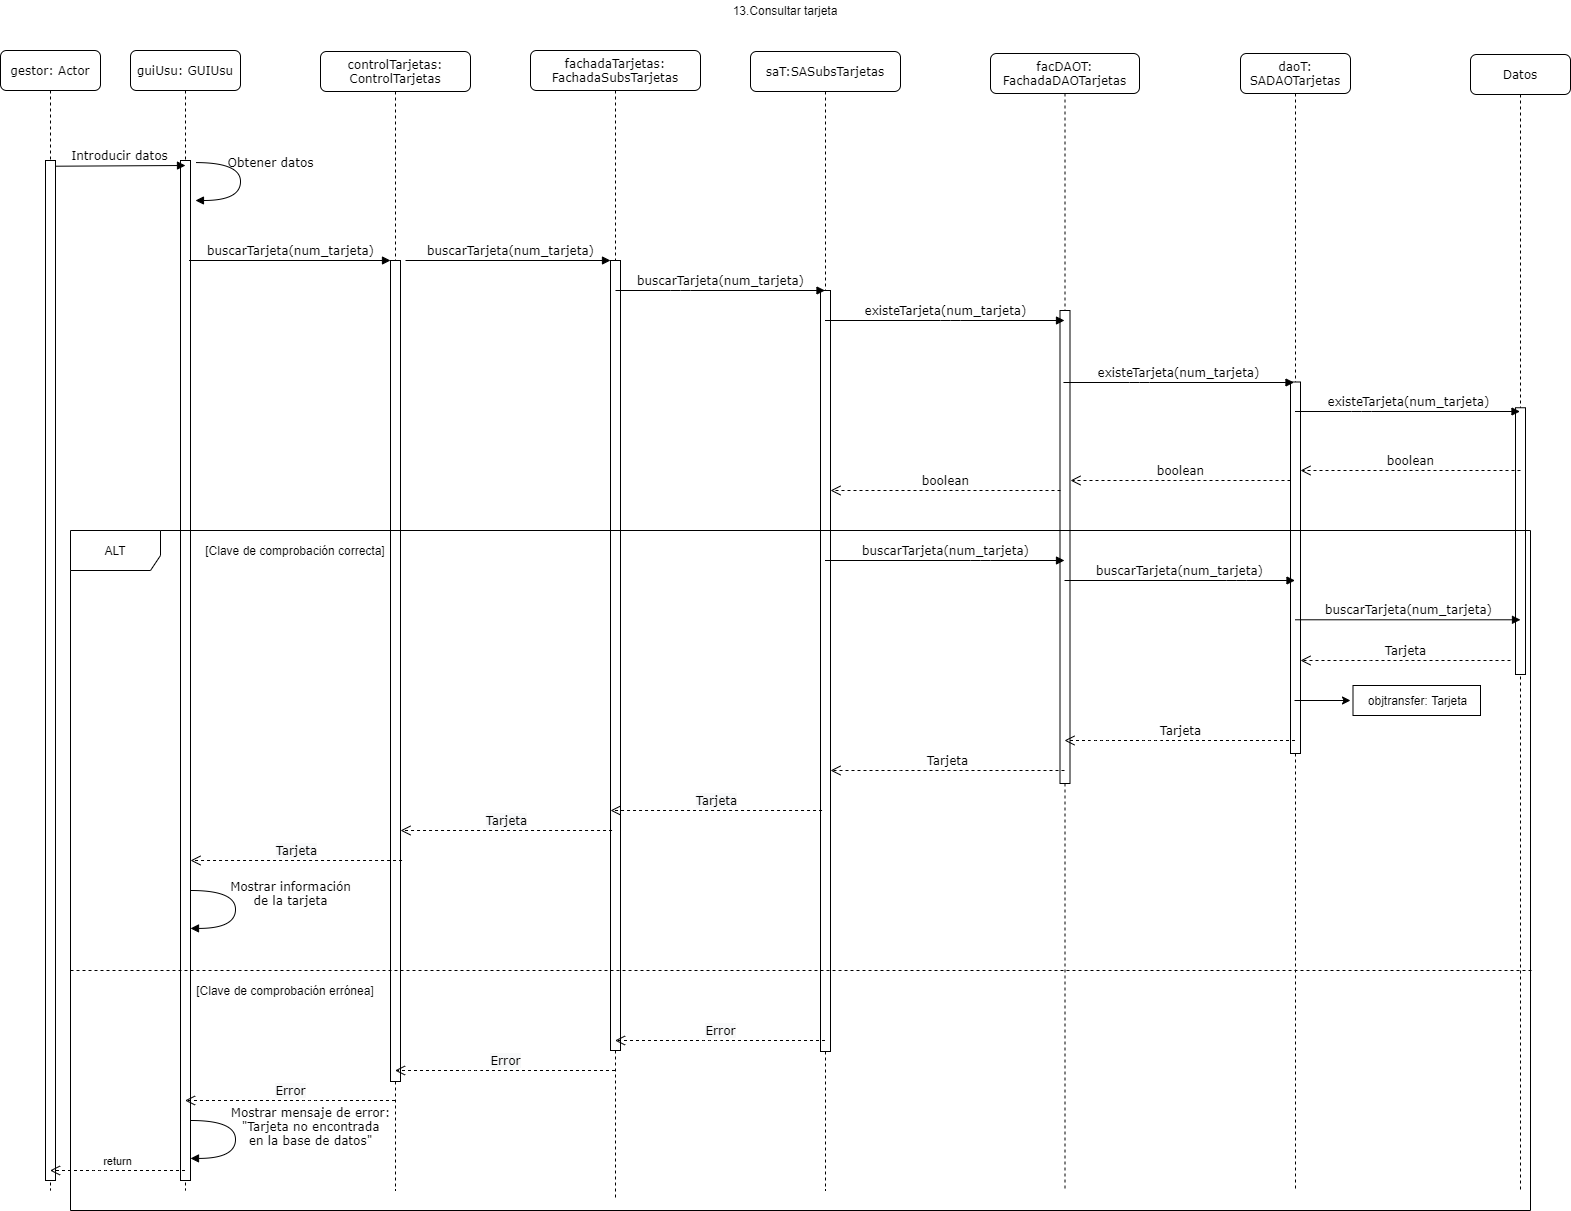
\includegraphics[width=0.8\textwidth]{images/consultarTarjeta.png}
\end{figure}
\subsection{Crear tarjeta}
\begin{figure}[H]
    \centering
    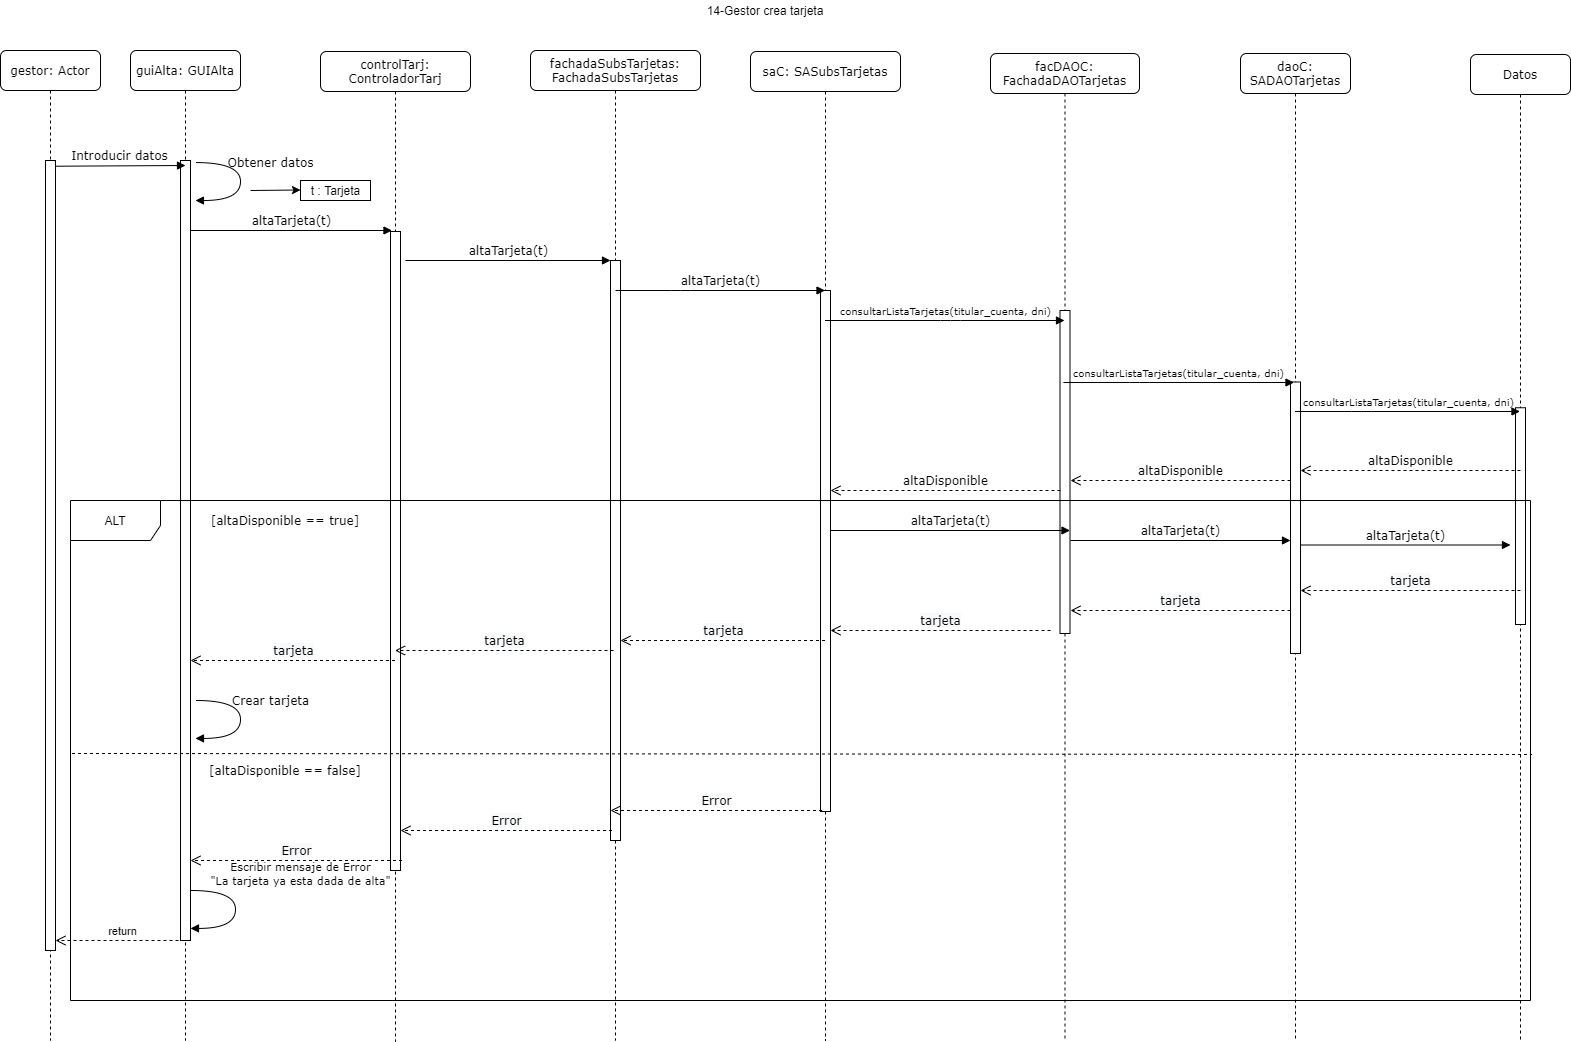
\includegraphics[width=0.8\textwidth]{images/14-Gestor_crea_tarjeta.png}
\end{figure}
\subsection{Eliminar tarjeta}
\begin{figure}[H]
    \centering
    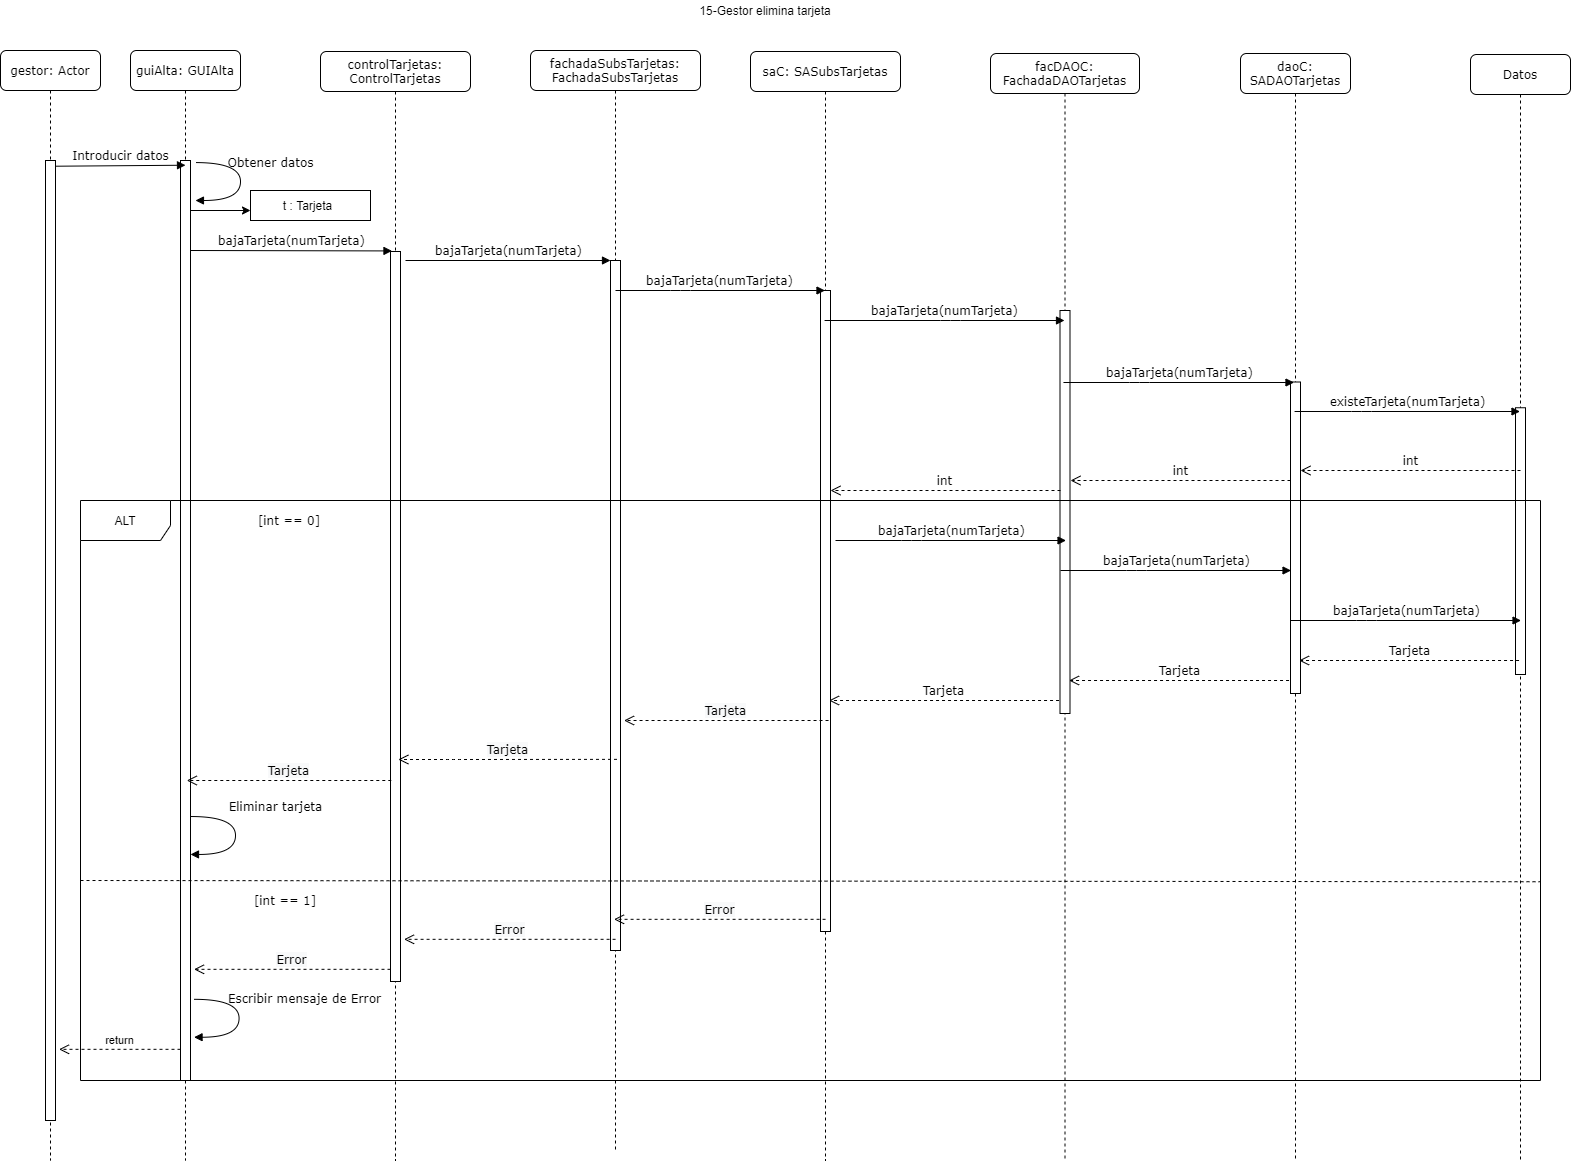
\includegraphics[width=0.8\textwidth]{images/15-Gestor_elimina_tarjeta.png}
\end{figure}
\subsection{Consultar lista de cuentas}
\begin{figure}[H]
    \centering
    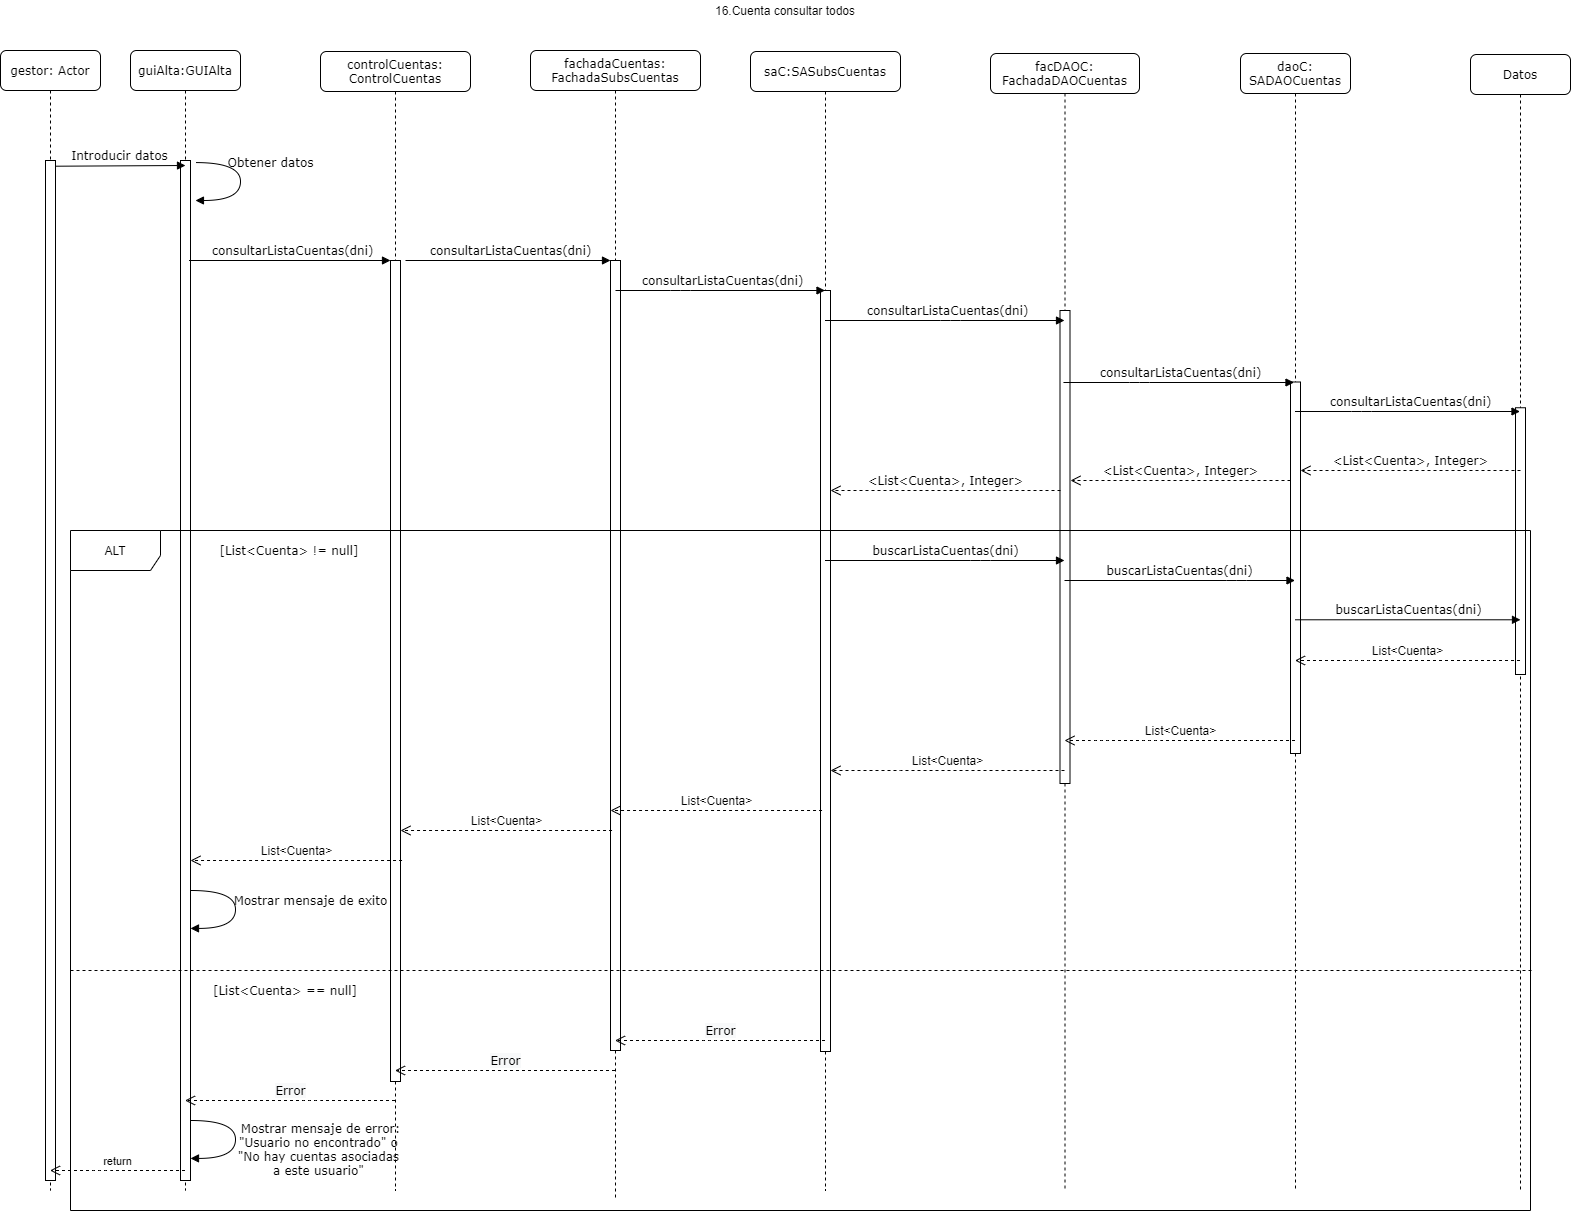
\includegraphics[width=0.8\textwidth]{images/16-cuentaconsultartodos.png}
\end{figure}
\subsection{Consultar lista de tarjetas}
\begin{figure}[H]
    \centering
    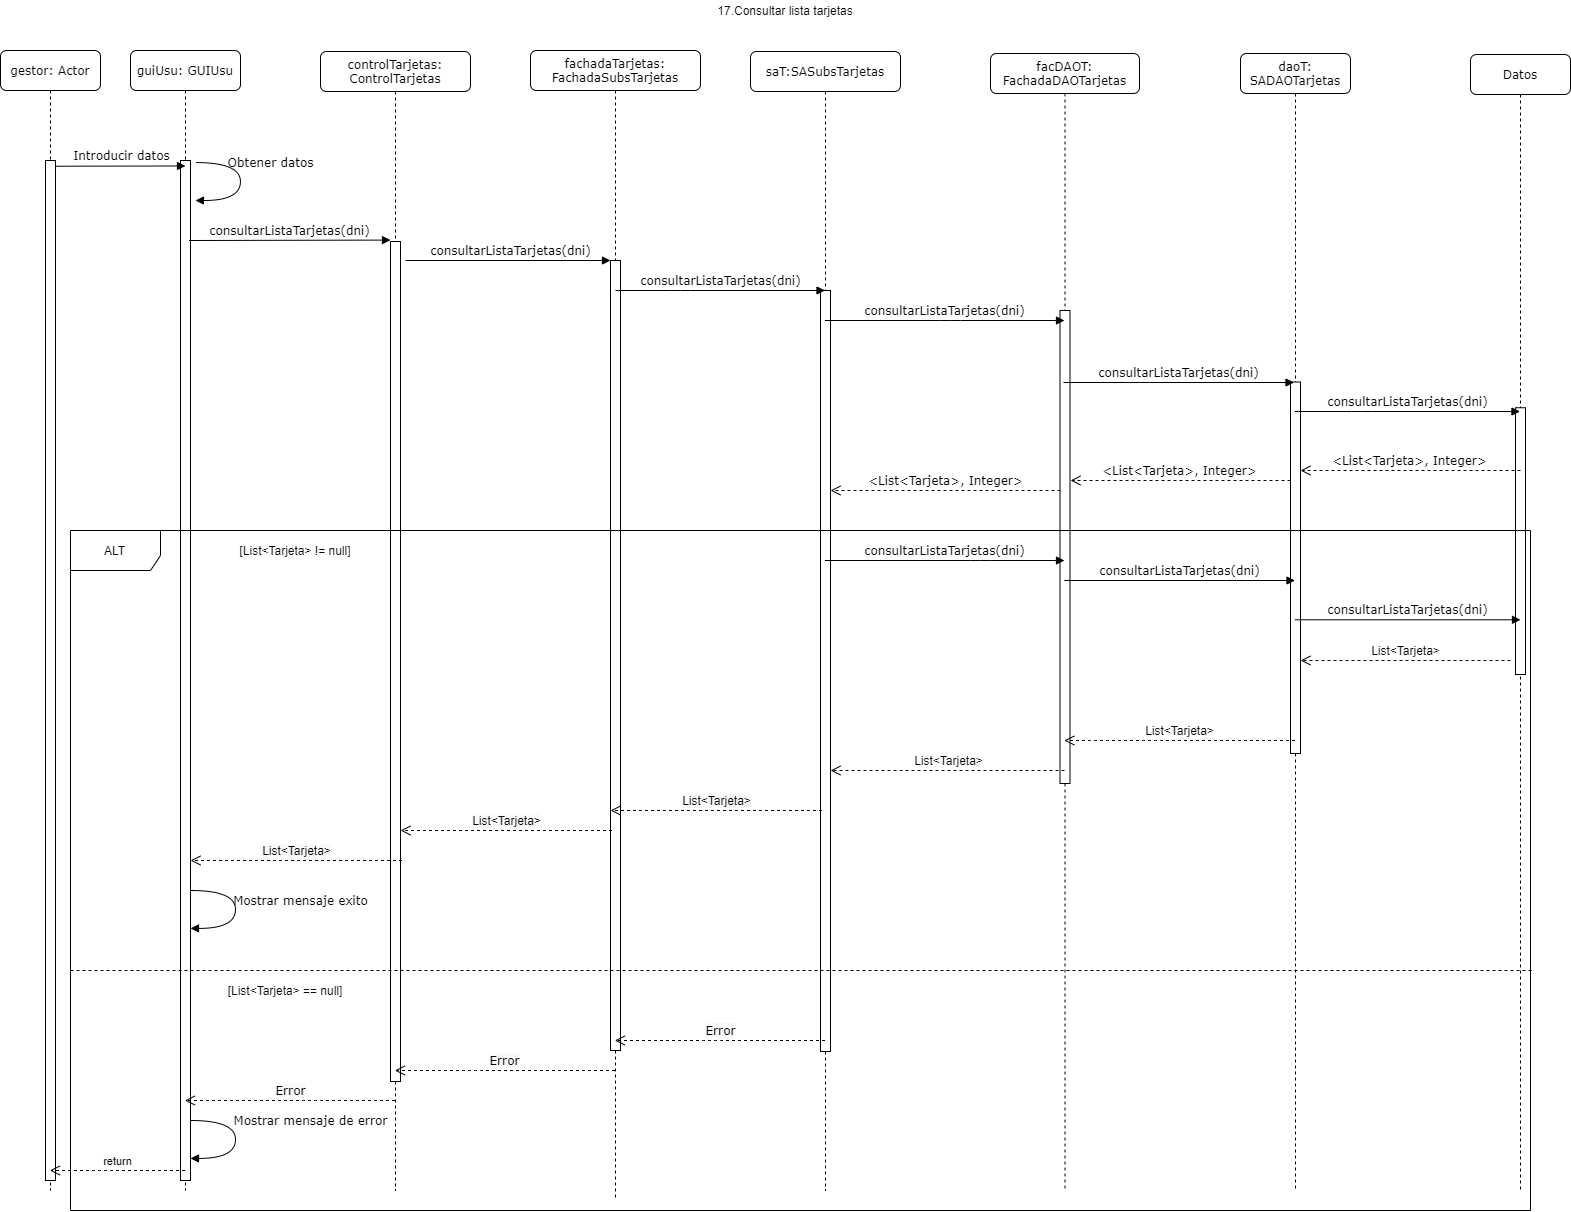
\includegraphics[width=0.8\textwidth]{images/consultarListaTarjetas.png}
\end{figure}
\subsection{Eliminar préstamo}
\begin{figure}[H]
    \centering
    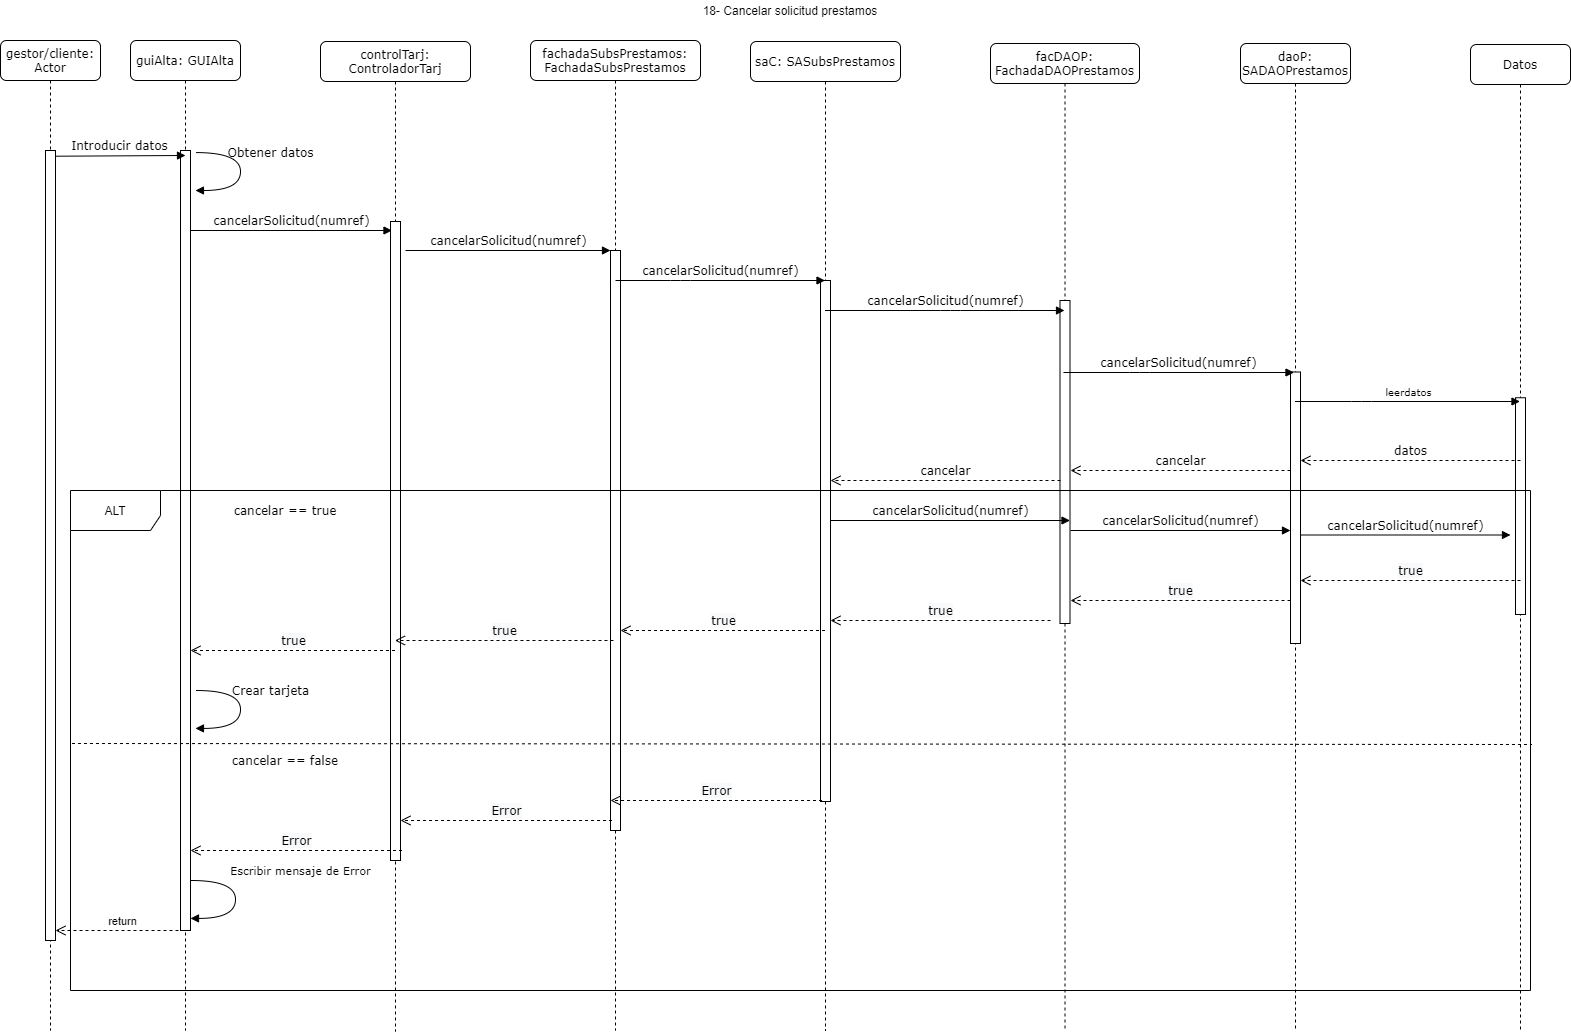
\includegraphics[width=0.8\textwidth]{images/18-eliminarprestamos.png}
\end{figure}
\subsection{Consultar lista de préstamos}
\begin{figure}[H]
    \centering
    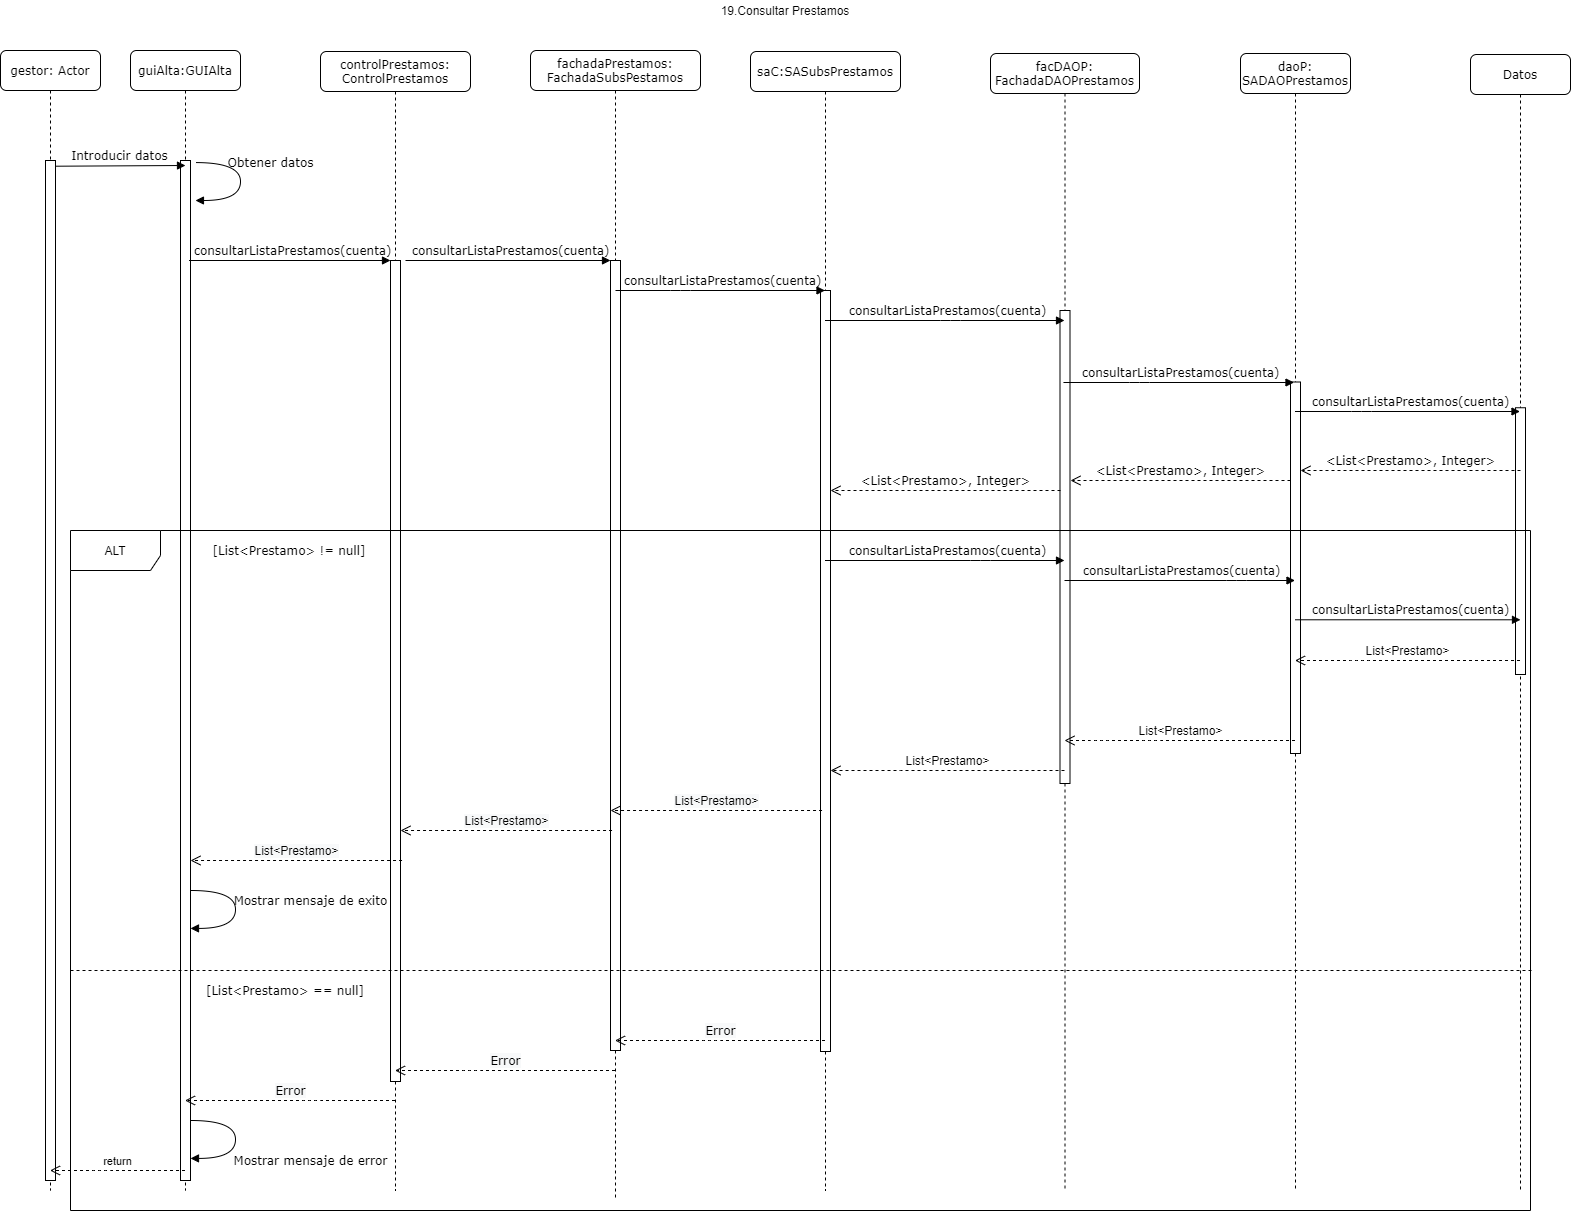
\includegraphics[width=0.8\textwidth]{images/19_consultar_prestamos.png}
\end{figure}
\subsection{Consultar lista de usuarios}
\begin{figure}[H]
    \centering
    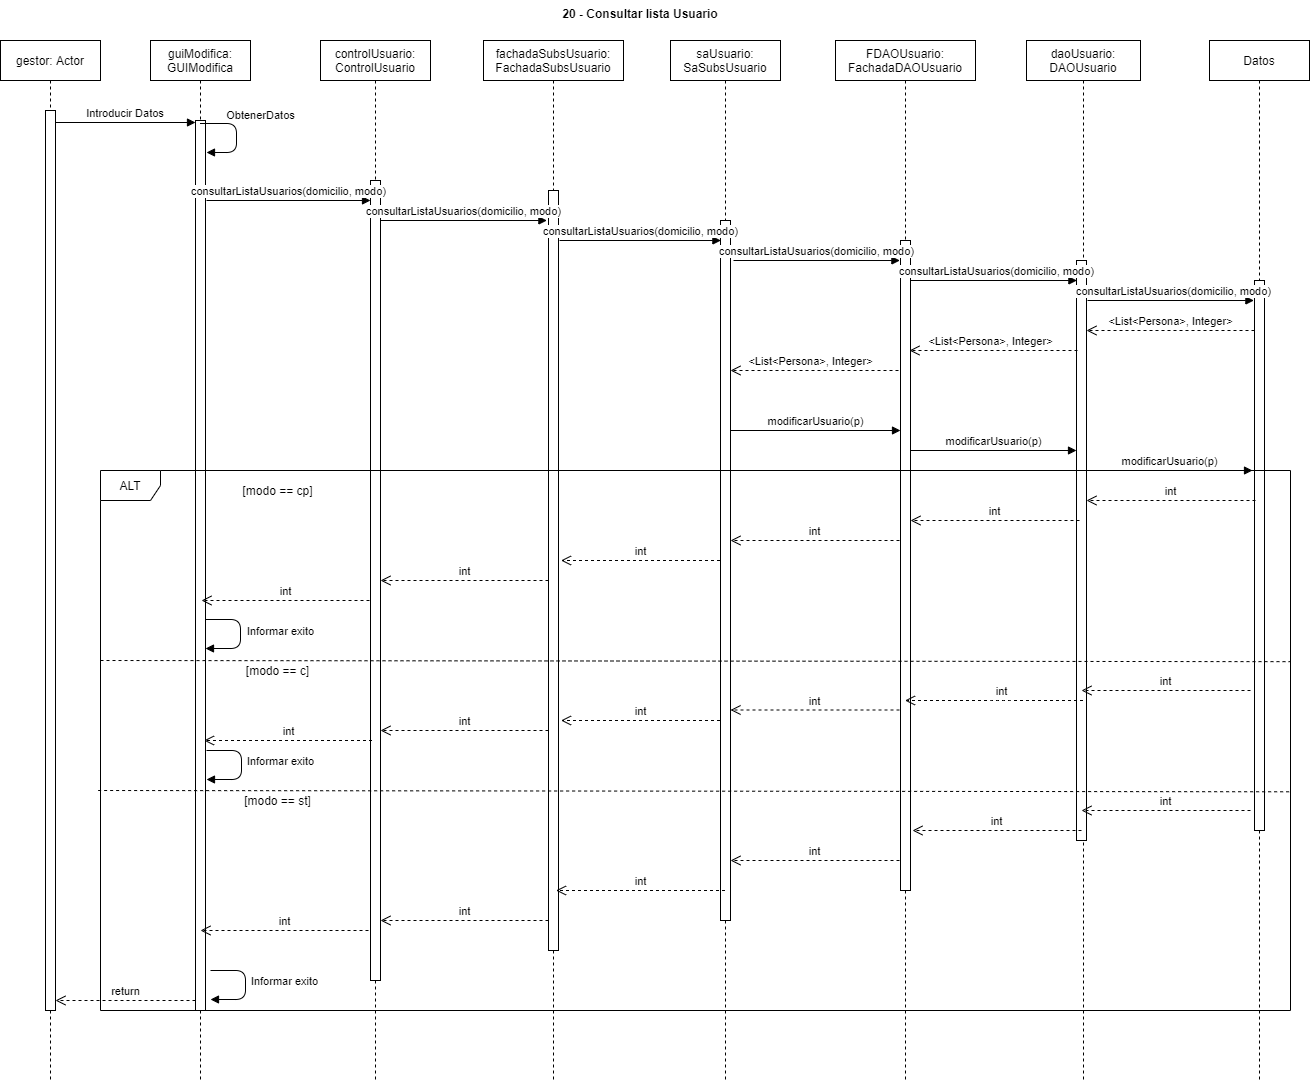
\includegraphics[width=0.8\textwidth]{images/20-consultarlistausuarios.png}
\end{figure}
\end{document}
